%%
%% Copyright 2019-2020 Elsevier Ltd
%%
%% This file is part of the 'CAS Bundle'.
%% --------------------------------------
%%
%% It may be distributed under the conditions of the LaTeX Project Public
%% License, either version 1.2 of this license or (at your option) any
%% later version.  The latest version of this license is in
%%    http://www.latex-project.org/lppl.txt
%% and version 1.2 or later is part of all distributions of LaTeX
%% version 1999/12/01 or later.
%%
%% The list of all files belonging to the 'CAS Bundle' is
%% given in the file `manifest.txt'.
%%
%% Template article for cas-dc documentclass for
%% double column output.

%\documentclass[a4paper,fleqn,longmktitle]{cas-dc}
\documentclass[a4paper,fleqn]{cas-dc}

%\usepackage[authoryear,longnamesfirst]{natbib}
%\usepackage[authoryear]{natbib}
\usepackage[numbers]{natbib}

%%%Author definitions
\def\tsc#1{\csdef{#1}{\textsc{\lowercase{#1}}\xspace}}
\tsc{WGM}
\tsc{QE}
\tsc{EP}
\tsc{PMS}
\tsc{BEC}
\tsc{DE}
%%%

%插入伪代码
\let\classAND\AND
\let\AND\relax
% load algorithmic
\usepackage{algorithmic}
\usepackage{algorithm}
\usepackage{subfig}

% save the new meaning of \AND and restore one of the class
\let\algoAND\AND
\let\AND\classAND
% but when we start \begin{algorithmic} we want its own \AND
\AtBeginEnvironment{algorithmic}{\let\AND\algoAND}

% \floatname{algorithm}{Algorithm}
\renewcommand{\algorithmicrequire}{\textbf{Input:}}
\renewcommand{\algorithmicensure}{\textbf{Output:}}
\renewcommand{\algorithmicendif}{\textbf{end}}


%调整断字
\hyphenpenalty=6000
\tolerance=700

%表格不要太宽
\usepackage{graphicx}
\usepackage{float}
\usepackage{url}
%表格斜线
\usepackage{diagbox}

\newdefinition{definition}{Definition}
\newtheorem{theorem}{Theorem}
\newtheorem{remark}{Remark}

\begin{document}




\let\WriteBookmarks\relax
\def\floatpagepagefraction{1}
\def\textpagefraction{.001}
\shorttitle{Surface--Subsurface
Observation of Tropical Cyclones}
\shortauthors{Yihui Ding et~al.}

\title [mode = title]{Multi-Agent Reinforcement Learning for Surface--Subsurface Observation of Tropical Cyclones Using Submersible Unmanned Vessels}
% \tnotemark[1,2]

% \tnotetext[1]{}

% \tnotetext[2]{}



\author[1,2]{Yihui Ding}[orcid=0009-0009-4133-1571]
\fnmark[1] % 添加脚注标记 1
\author[1,2,3]{\hspace*{0.33em}Xiwen Ma}[orcid=0000-0001-9212-3523]
\fnmark[1] % 添加脚注标记 1
\author[1,2]{\hspace*{0.33em}Wenlei Peng}
\author[1,2,4]{\hspace*{0.33em}and\hspace*{0.33em}Jingsong Yang}[orcid=0000-0002-7514-3212]
\cormark[1]

\address[1]{School of Oceanography, Shanghai Jiao Tong University, Shanghai, 200030, China}
\address[2]{State Key Laboratory of Satellite Ocean Environment Dynamics, Second Institute of Oceanography, Ministry of Natural Resources, Hangzhou, 310012, China}
\address[3]{Institute of Automation Chinese Academy of Sciences, Beijing, 100190, China}
\address[4]{Southern Marine Science and Engineering Guangdong Laboratory (Zhuhai), Zhuhai, 519082, China}
\fntext[1]{These authors contributed equally to this work.}
\cortext[1]{Corresponding author: Jingsong Yang. Email: \tt{jsyang@sio.org.cn}}

\begin{abstract}
Tropical cyclones remain destructive, while intensity and rapid-intensification
forecasts are constrained by sparse near-core observations. Conventional
platforms rarely combine rapid transit, surface-wind sampling, and
subsurface-current sensing. We develop and evaluate a simulation-based
multi-agent reinforcement learning framework for surface--subsurface TC
observation using parameterized Blue Whale-class submersible unmanned vessels.
Event-specific environments combine ERA5 10 m winds, HYCOM currents from 0--60
m, and IBTrACS tracks for 500 western North Pacific TCs. A parameter-sharing
IPPO policy maps local observations to continuous commands every 10 min.
Center distance is used only in training; validation tests frozen policies on
unseen TCs using shared winds. Surface vehicles correct deployment errors and
approach the high-wind region; underwater, they sample currents at seven
depths. Ten seeds cover 4/8/12/16 vehicles at 12 and 20 m/s and validation
radii of 100--800 km. Time-averaged tracking distance is lower at 20 m/s in all
20 fleet-size/radius comparisons; the fleet-averaged gap grows from 10.1 to
84.2 km. The 12 m/s scenario uses shorter paths and lower speed, revealing an
efficiency--tracking trade-off. Low-pass filtering improves final tracking on
average while shortening trajectories and reducing peak speed. Underwater
experiments compare active IPPO, random control, and passive drift at seven
depths. The surface results support active tracking; the subsurface tests
quantify whether propulsion improves current sampling over drift.
\end{abstract}

% \begin{graphicalabstract}
% \includegraphics{figs/grabs.pdf}
% \end{graphicalabstract}

\begin{highlights}
\item Dual-mode SUVs track surface winds and sample subsurface currents.
\item Event-specific ERA5--HYCOM environments cover 500 historical TCs.
\item Parameter-sharing IPPO is evaluated for 4- to 16-SUV fleets.
\item Underwater experiments compare active, random, and passive-drift control.
\end{highlights}

\begin{keywords}
tropical cyclone observation \sep submersible unmanned vessel \sep
multi-agent reinforcement learning \sep
surface--subsurface observation
\end{keywords}

\maketitle

\section{Introduction}
Tropical cyclones are among the most destructive manifestations of extreme
weather. Their strong winds, extreme rainfall, storm surges, and waves threaten
lives, coastal infrastructure, fisheries, shipping, and offshore operations.
Recent assessments and attribution studies indicate that the global number of
TCs may not increase uniformly, but the proportion of intense storms, rapid
intensification events, rainfall extremes, and destructive potential has
increased in many basins \citep{r1,r2,r3,r4}. Over the western
North Pacific, landfalling TCs have intensified since the late 1970s, and the
destructive potential of landfalling TCs over China has increased
\citep{r5,r6}. Nearshore intensification and the migration of TC activity
toward higher latitudes and populated coastlines further increase risk in East
Asia and the East China Sea \citep{r7,r8}. Consequently, improved prediction
of TC track, intensity, wind radii, and upper-ocean response is an urgent
requirement for disaster risk reduction.
Track forecasting has improved substantially through better numerical weather
prediction, satellite data assimilation, ensemble design, and, more recently,
data-driven global weather models. Intensity forecasting has advanced more
slowly \citep{r9,r10}. A central reason is that intensity is controlled not only
by the large-scale atmospheric environment but also by air--sea enthalpy and
momentum exchange, upper-ocean heat content, barrier-layer thickness, cold
wakes, mesoscale eddies, and TC-induced currents. Strong winds mix the upper
ocean, generate near-inertial currents, cool the sea surface, deepen the mixed
layer, and modify vertical thermal and salinity structure; these responses feed
back on surface fluxes and subsequent intensification \citep{r11,r12}.
Satellite observations provide broad spatial coverage, but clouds and rain
attenuate microwave signals, scatterometers saturate at high winds, and
spaceborne products cannot directly resolve the subsurface ocean. The near-core
wind and upper-ocean state therefore remain insufficiently constrained in many
forecast initial conditions.
Another challenge is the mismatch between the scales of the atmospheric and oceanic observing systems. The TC core and eyewall evolve over tens of kilometers and hours, whereas global atmospheric reanalyses and operational analyses are commonly available at quarter-degree and hourly resolution. Upper-ocean models provide finer horizontal grids, but assimilated observations are still spatially sparse. Even when temperature and salinity profiles are available, their forecast impact depends on where and when they are collected relative to the storm, the pre-existing barrier layer, and the ocean eddy field. Observations that are late, far from the sensitive region, or redundant with neighboring measurements may have little influence on the analysis. Adaptive observation is therefore not simply a coverage problem; it is a sequential decision problem involving motion, sampling time, energy, and coordination.

Current TC observing systems can be grouped into remote sensing, airborne,
anchored, drifting, and autonomous underwater platforms \citep{r13,r14,r15}.
Satellites are indispensable for monitoring storm position, cloud structure,
precipitation, sea surface temperature, and large-scale winds \citep{r13}.
They offer repeat coverage and synoptic context but cannot simultaneously
resolve the surface wind maximum, the wave field, and the three-dimensional
upper ocean beneath the core. Manned aircraft and dropwindsondes provide
high-quality boundary-layer, eyewall, and upper-ocean information, but they are
expensive, weather dependent, and limited to relatively short campaigns
\citep{r14}. Small uncrewed aircraft can sample the turbulent eyewall boundary
layer, but remain short-duration and range-limited \citep{r15}. Fixed moorings
and buoys provide accurate time series but cannot follow a moving storm.
Surface drifters sample Lagrangian pathways but provide little control over
where measurements are made. Underwater gliders can remain at sea for weeks and
have demonstrated value in TC research and assimilation, but their
buoyancy-driven speed is much lower than storm translation speed
\citep{r16,r17}. Wave gliders and conventional autonomous surface vehicles can
communicate more easily, but they do not directly sample the subsurface current
and stratification.
The observational value of underwater platforms has nevertheless been
demonstrated. Assimilation of glider profiles can improve the upper-ocean
initial state and, in some cases, TC intensity forecasts \citep{r18,r19}.
Strongly coupled ocean--atmosphere assimilation allows ocean observations to
influence atmospheric analyses through cross-domain error covariances
\citep{r20}. Studies using hypothetical current-observing networks and Marine
JEDI show that current observations can alter coupled states and TC
forecasts \citep{r21,r22}. The benefit is highly sensitive to the observing
location and background ocean structure \citep{r23,r24,r25}. This motivates
platforms that can move rapidly toward the predicted TC, adapt their
sampling paths in response to local measurements, and switch between surface
and subsurface operation.

A submersible unmanned vessel (SUV) combines characteristics of an unmanned surface vehicle and a submersible. It can use conventional propulsion for rapid surface transit, then lower the main hull below the free surface for improved seakeeping, sensor stability, and subsurface sampling \citep{r28,r29,r30,r31}. The Blue Whale, developed by the Second Institute of Oceanography, Ministry of Natural Resources, China, is an engineering reference for this class of platform \citep{r28}. It uses surface propulsion, four vector thrusters for low-speed subsurface maneuvering, and ballast, anchoring, and center-of-gravity control for submerged station keeping. Its public specifications include a maximum surface speed of about 23 kn (11.83 m/s), a submerged speed of about 3 kn (1.54 m/s) for at least 4 h, submerged standby for at least 72 h, a reference depth of about 60 m, and a minimum payload of about 800 kg. It can carry current profilers, CTD and biogeochemical sensors, and a rocketsonde for atmospheric profiles.
This study does not attempt a digital twin of the current Blue Whale. Instead, the current platform provides the engineering baseline, and a future Blue Whale-class parameterization extends surface speed, endurance, depth, communication, and payload within explicitly identifiable scenarios. This distinction is important: an improved propulsion or energy system may be studied without attributing unverified performance to the present vehicle. The platform model represents speed, endurance, sampling depth, communication, energy, and safety constraints, while deliberately omitting high-fidelity hull hydrodynamics, wave loads, and actuator response.

The proposed observation cycle uses two coupled operating modes. In surface
mode, the fleet moves rapidly toward the TC and enters the high-wind region.
In subsurface mode, the vehicles dive to sampled depths and observe the
TC-conditioned current field. The measured variables are therefore explicitly
separated: at the sea surface, the SUVs observe wind speed and direction at
10 m above the sea surface; below the sea surface, they observe the horizontal
current velocity components and the derived current speed at depths from 0 to
60 m. Figure~\ref{fig:system_architecture} illustrates this transition. Four
vehicles are used as the visual example, with equal angular spacing; the
subsequent experiments extend the same parameter-sharing policy to 8, 12, and
16 vehicles. The stages share the platform and event data but are evaluated as
separate tasks: the surface endpoint defines the operational handoff to the
underwater rollout, while the dynamic dive, ballast, and resurfacing processes
are outside the present motion model.

\begin{figure*}[htbp]
\centering
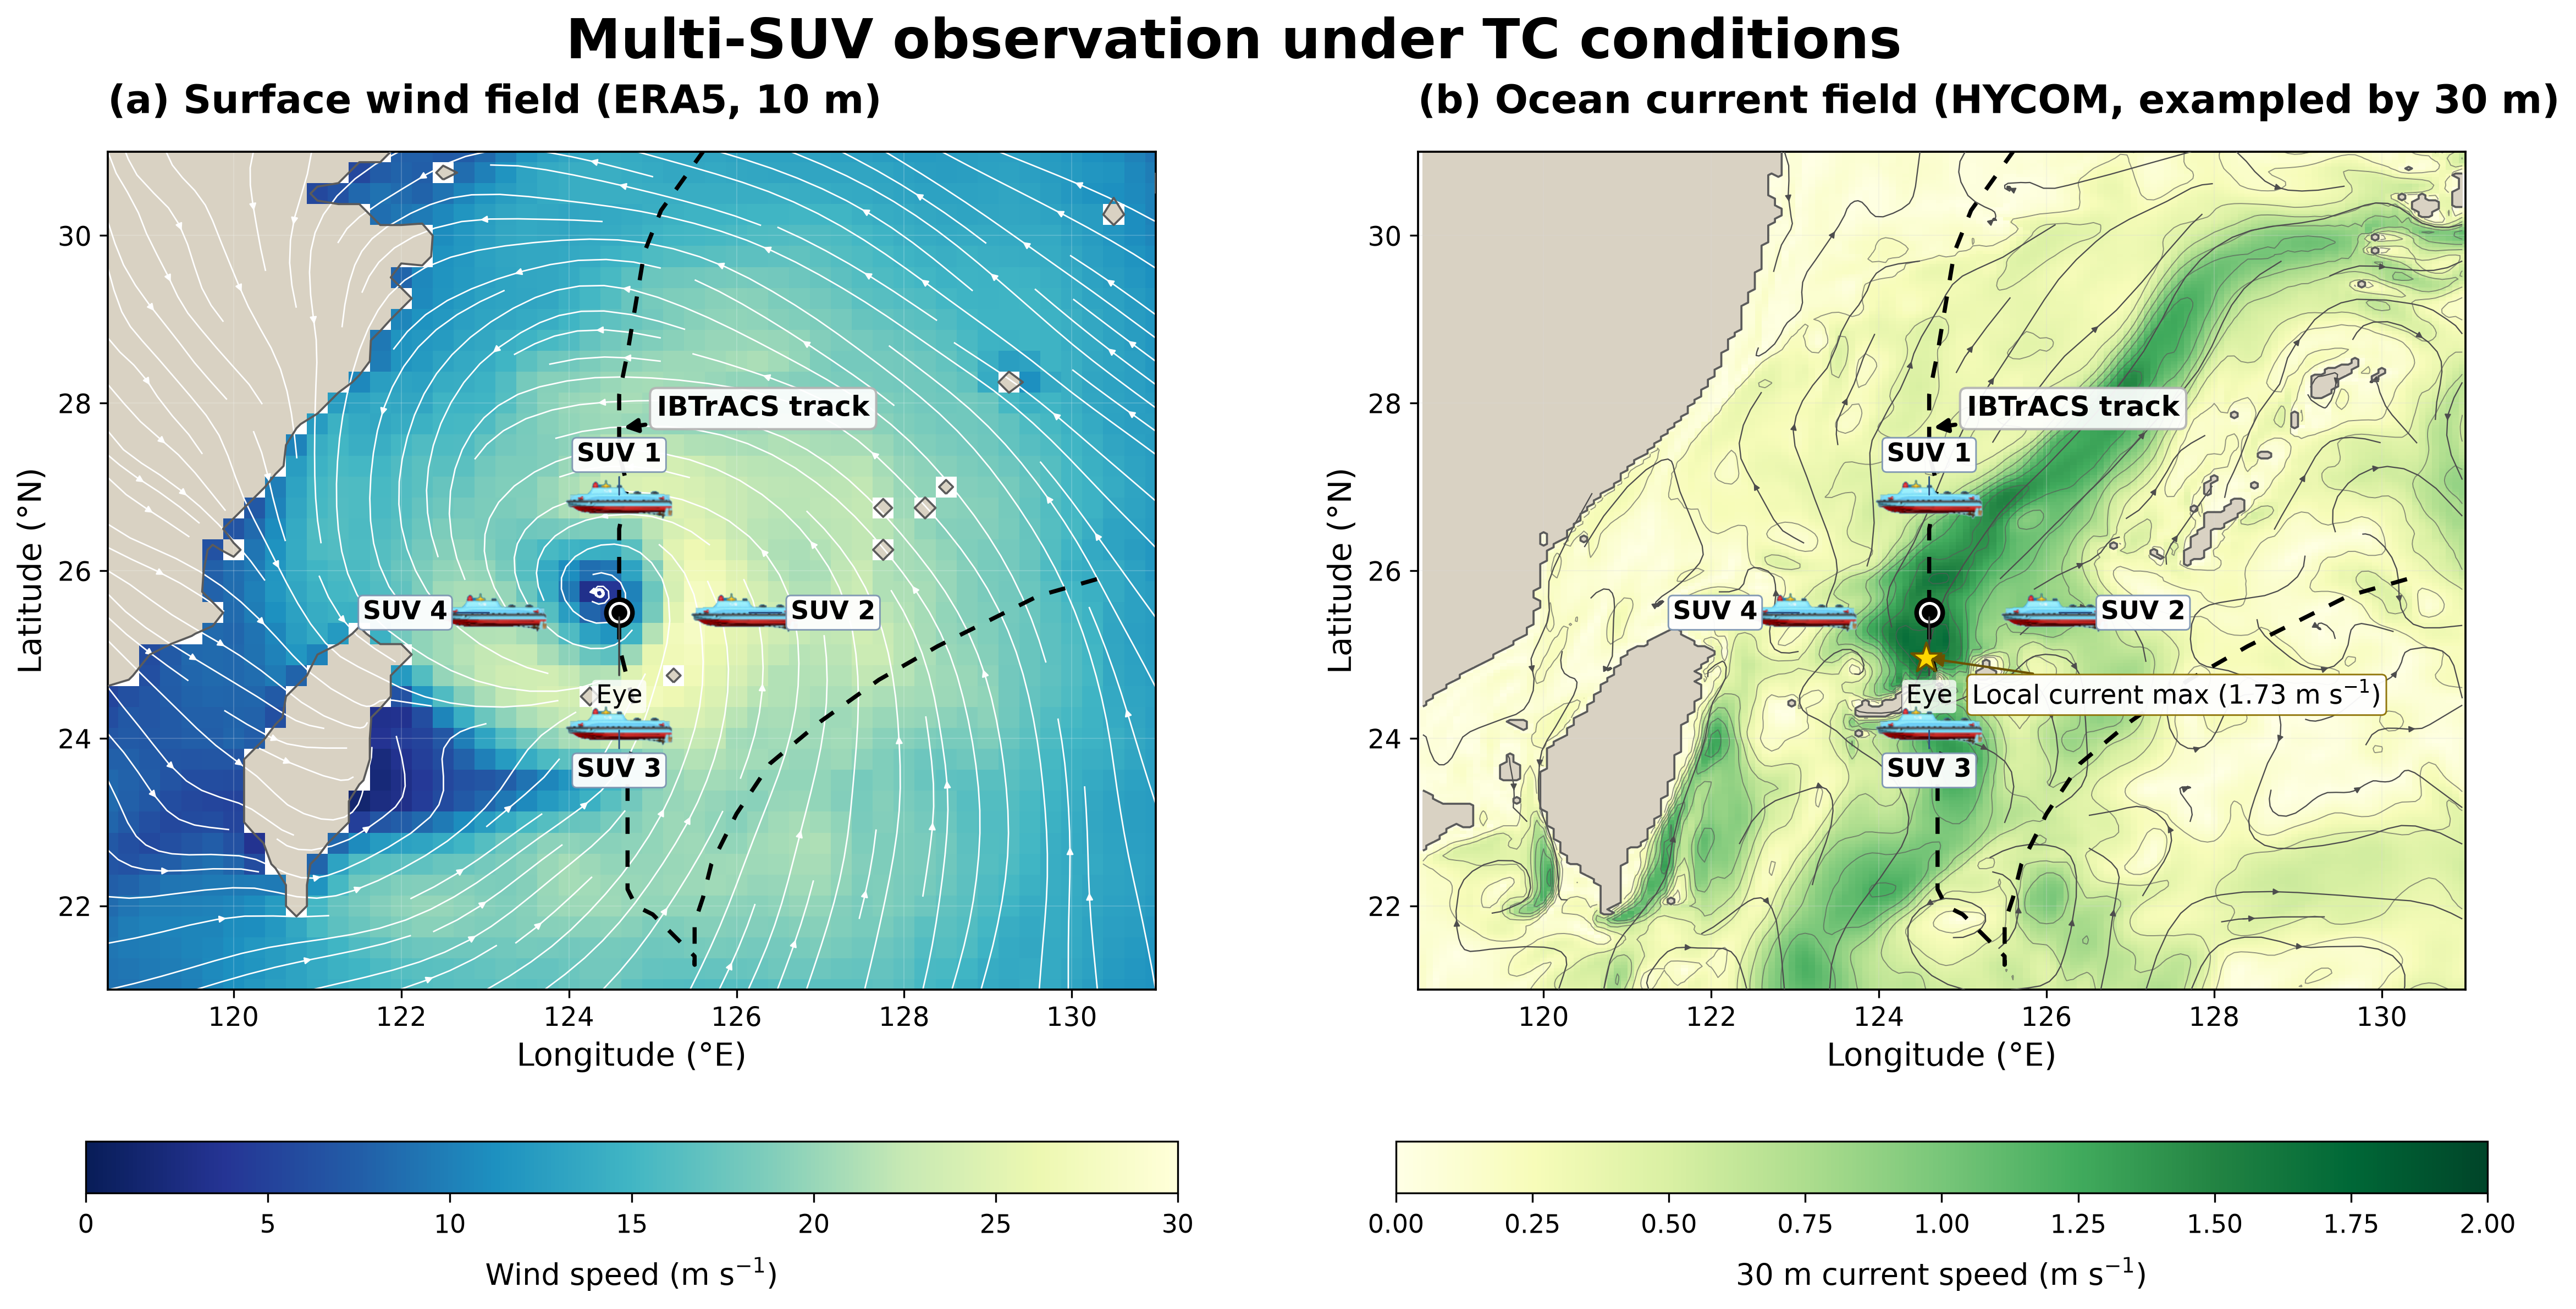
\includegraphics[width=\textwidth]
    {figures/fig2_surface_subsurface_observation.png}
\caption{Coordinated surface--subsurface TC observation for a representative
HINNAMNOR (2022) snapshot. The left panel shows four SUVs tracking the IBTrACS
best track while sampling ERA5 winds at 10 m above the sea surface. The right
panel shows the same formation sampling HYCOM currents at 30 m below the sea
surface; this depth is shown as an illustrative example, whereas the complete
experiments cover the seven depths from 0 to 60 m. The four-vehicle
configuration is illustrative, with equal angular spacing; subsequent
experiments evaluate fleets of 8, 12, and 16 vehicles.}
\label{fig:system_architecture}
\end{figure*}

Classical graph-search, sampling-based, potential-field, and model predictive control methods have been used extensively for autonomous vehicle planning. Dijkstra and A* obtain optimal paths on known cost graphs, A* uses a heuristic to reduce search effort, and D* Lite repairs a previous solution when edge costs change \citep{r43,r44}. RRT and RRT* handle high-dimensional and nonholonomic constraints and approach feasible or asymptotically optimal solutions through sampling \citep{r45}. Artificial potential fields are computationally efficient but can become trapped in local minima \citep{r46}. Model predictive control explicitly handles dynamics, energy, and obstacle constraints over a receding horizon, but requires a reliable prediction model and repeated online optimization \citep{r47}. A comprehensive review of AUV planning is given by Panda et al. \citep{r48}. These methods remain valuable when the cost map and dynamics are known. In a TC environment, however, the wind and current fields vary continuously, vehicle ground velocity is the superposition of propulsion and ambient flow, and the moving cost graph would need frequent reconstruction. Each vehicle observes only a local patch, while multiple vehicles are coupled through coverage, redundancy, communication, and coastal safety.
Traditional planning pipelines often decouple observation from path
generation: a field estimate, cost map, or waypoint sequence is first
constructed and then executed. In the RL formulation used here, the current
measurement directly enters the policy state and changes the next action; that
action changes the vehicle position and produces a new measurement. Observation
and motion planning are therefore coupled in one feedback law rather than
treated as separate sequential modules.
Reinforcement learning provides an alternative for closed-loop decision making
under uncertainty. A policy is optimized through repeated interaction with the
environment and can approximate a state-to-action mapping without explicitly
solving the full stochastic transition model. RL has achieved strong results
in language-model alignment and reasoning \citep{r49,r50,r51}, legged
locomotion and dexterous manipulation \citep{r52,r53}, drone racing
\citep{r54}, and high-dimensional games \citep{r55,r56}. Independent PPO has
been competitive in cooperative multi-agent benchmarks and games
\citep{r41,r42}, including the StarCraft Multi-Agent Challenge \citep{r57}.
In the ocean domain, multi-AUV adaptive sampling and cooperative control are
established applications \citep{r32}; RL has more recently been applied to
underwater target tracking and cooperative AUV tasks \citep{r33,r34,r36}.
Hybrid adaptive methods also remain useful for multi-AUV cooperative hunting
in obstacle-rich environments \citep{r35}.

Three unresolved gaps motivate this study. First, previous planning studies
often reconstruct the ocean response with simplified analytical or
reduced-order flow models \citep{r26,r27} and therefore do not explicitly use
event-specific background eddies, fronts, vertical shear, or non-stationary
current structures. Second, TC track forecasts retain
finite position and timing errors \citep{r23,r24,r25}; fixed pre-deployment and
waiting strategies can therefore miss the actual high-wind region. A practical
system must allow the fleet to move rapidly from its deployment location to
the high-wind region and then descend for subsurface sampling. Third, the
closest previous multi-AUV active-observation study used four vehicles
\citep{r27}; fleet-size sensitivity therefore remains insufficiently explored,
limiting the number of simultaneous and spatially distributed observations.
The present study therefore evaluates four fleet sizes: 4, 8, 12, and 16 SUVs.

From a control perspective, the coupled wind--current environment is
nonstationary, spatially heterogeneous, and stochastic. Exact online solution
of the full multi-agent transition model is therefore impractical under partial
observability and limited computation. We formulate the decision problem as
stochastic-approximation-based policy optimization, in which neural networks
approximate the policy and value functions. IPPO learns the closed-loop policy
from repeated interaction with event-specific environmental fields
\citep{r40,r41,r42}.
Three earlier results define the starting point of this work. Qi et al.
developed a forecast-path correction model that used AUV current observations
to infer TC information and update a tracking path \citep{r26}. A subsequent
multi-AUV active observation framework included forecast tracks, background
currents, travel time, energy, and redundancy, but represented the ocean with
an analytical model \citep{r27}. These studies provide the center-inference and
task-planning foundations for the present work; the event-specific
surface--subsurface loop developed here addresses the gaps identified above.



\section{Problem Formulation }\label{sec:problem}

\subsection{Observation Task and Design Requirements}

The objective is to coordinate a fleet of submersible unmanned vessels
(SUVs) to observe a moving tropical cyclone (TC) across the sea surface and
upper ocean. Each SUV first navigates on the surface toward the predicted TC
center and high-wind region. After entering a predefined high-wind observation
window, the fleet descends to a specified depth and samples the TC-induced
current field. The framework is designed to satisfy four operational requirements:

\begin{enumerate}
\item rapid correction of initial deployment errors using surface propulsion;
\item decentralized tracking of the moving TC using onboard wind observations
and inter-vehicle observation sharing;
\item subsurface observation at ocean depths of 0, 10, 20, 30, 40, 50, and
60 m below the sea surface;
\item safe operation under propulsion-energy, communication, action-smoothness,
and coastline constraints.
\end{enumerate}

The surface maximum speed is varied between 12 and 20 m/s, while the submerged
maximum propulsion speed is 1.5 or 2.0 m/s. This difference creates an asymmetric
decision problem: active propulsion is necessary at the surface, whereas
underwater observation must also consider passive advection by the ambient
current.

\subsection{Problem Definition}

The fleet contains $N$ SUVs, where $N\in\{4,8,12,16\}$, indexed by
$i\in\{1,2,\ldots,N\}$. The position, propulsion velocity,
and operating mode of SUV $i$ at time $t$ are denoted by
$\mathbf{x}_i(t)$, $\mathbf{p}_i(t)$, and $m_i(t)\in\{\mathrm{s},\mathrm{u}\}$,
respectively, where $\mathrm{s}$ and $\mathrm{u}$ denote the surface and
subsurface modes. The propulsion speed satisfies
\begin{equation}
\|\mathbf{p}_i(t)\|\leq
\begin{cases}
V_{\max}^{\mathrm{s}}, & m_i(t)=\mathrm{s},\\
V_{\max}^{\mathrm{u}}, & m_i(t)=\mathrm{u}.
\end{cases}
\label{eq:speed_constraint}
\end{equation}

The horizontal motion of the SUV is modeled as
\begin{equation}
\dot{\mathbf{x}}_i(t)=
\begin{cases}
\mathbf{p}_i(t), & m_i(t)=\mathrm{s},\\[1mm]
\mathbf{p}_i(t)+
\mathbf{u}_{\mathrm{ocean}}
\left(\mathbf{x}_i(t),z_i,t\right), & m_i(t)=\mathrm{u},
\end{cases}
\label{eq:platform_motion}
\end{equation}
where $z_i\in\{0,10,20,30,40,50,60\}$ m and
$\mathbf{u}_{\mathrm{ocean}}(\cdot)$ is the HYCOM current at the corresponding
position and depth. Thus, the underwater ground velocity is the superposition of
active propulsion and background advection.

For numerical implementation, the continuous model is integrated explicitly at
the decision interval $\Delta t=10$ min:
\begin{equation}
\mathbf{x}_{i,k+1}=
\begin{cases}
\mathbf{x}_{i,k}+\mathbf{p}_{i,k}\Delta t,
& m_{i,k}=\mathrm{s},\\[1mm]
\mathbf{x}_{i,k}+
\left[
\mathbf{p}_{i,k}+
\mathbf{u}_{\mathrm{ocean}}(\mathbf{x}_{i,k},z_i,t_k)
\right]\Delta t,
& m_{i,k}=\mathrm{u}.
\end{cases}
\label{eq:platform_motion_discrete}
\end{equation}
The current field is evaluated at the beginning of each interval and
interpolated to the current vehicle position.
For the active underwater reward, we write this pre-move current as
$\mathbf{u}_{i,k}=\mathbf{u}_{\mathrm{ocean}}
(\mathbf{x}_{i,k},z_i,t_k)$.

This equation is deliberately a reduced-order horizontal point-mass
kinematic--advection model rather than a six-degree-of-freedom rigid-body
dynamic model. It does not resolve added mass, hydrodynamic drag, roll, pitch,
yaw or heading dynamics, buoyancy and ballast dynamics, thruster transients,
wave loads, or actuator delay. This simplification is consistent with the
information content of the environmental forcing. ERA5 winds are available at
$0.25^\circ$ and hourly resolution, whereas HYCOM currents are available at
approximately $0.04^\circ$ by $0.08^\circ$ and three-hourly resolution. These
fields are interpolated to the 10 min decision interval and to each vehicle
position, but such interpolation does not recover high-frequency wave forcing,
local wake effects, or unobserved vehicle attitude and actuator states.
Introducing a detailed six-degree-of-freedom model would therefore require
platform-specific hydrodynamic coefficients and forcing information that are
not commensurate with the present data, and could imply a level of numerical
precision unsupported by the inputs. The reduced model retains the first-order
effects relevant to mission-level planning: mode-dependent speed limits,
propulsion commands, ambient-current advection in subsurface mode, and coastal
constraints. Accordingly, the results are interpreted as mission-planning and
coordination evidence rather than as predictions of attitude, structural
loading, or low-level controller response. Coupling this planning layer to an
experimentally calibrated six-degree-of-freedom vehicle model is left for future work.

The local observation of SUV $i$ is
\begin{equation}
\mathbf{o}_i(t)=
\left[
\mathbf{s}_i(t),
\mathbf{v}_i(t),
\mathbf{h}_i(t)
\right],
\label{eq:observation}
\end{equation}
where $\mathbf{s}_i(t)$ contains the observation used in the corresponding
stage and $\mathbf{v}_i(t)$ is the normalized commanded propulsion velocity,
$\mathbf{v}_i=\mathbf{p}_i/V_{\max}^{m_i}$; it is not the total ground velocity.
In the final surface experiments, $\mathbf{s}_i(t)$ consists only of the
normalized wind patches at 10 m above the sea surface sampled by the $N$ SUVs,
and no historical frame is used. Surface operation assumes idealized, lossless,
and instantaneous inter-vehicle communication: every SUV receives the wind observations acquired
by all other SUVs in the fleet as part of its policy input. In the underwater
active-control comparison, no inter-vehicle communication is assumed.
Accordingly, $\mathbf{s}_i(t)$ consists only of SUV $i$'s local current speed
and components at its assigned ocean depth, while $\mathbf{h}_i(t)$ contains a
five-frame history of that same vehicle's local current. Each underwater SUV
therefore knows neither the current observations nor the positions or actions
of the other SUVs. The complete reanalysis field, the global best-track center,
and future environmental states are not provided to the policy.
Accordingly, the surface observation dimension is $d_o^{\mathrm{s}}=3N+2$.
The underwater active controller uses a $1\times1$ local-current observation
plus a five-frame history and two normalized propulsion components, giving
$d_o^{\mathrm{u}}=5\times3+2=17$.

During training, the reward function can access the distance between each SUV
and the best-track TC center. This distance supervises the association between
local 10 m wind patterns and proximity to the TC center/high-wind region; the
center coordinate itself is not an actor input. During validation, rewards do
not influence actions. The frozen policy receives only the shared fleet-level
wind samples and must track an unseen TC, thereby testing whether the learned
wind-to-center relation generalizes.

The normalized action is
\begin{equation}
\mathbf{a}_i(t)\in[-1,1]^2,
\end{equation}
and is projected onto the unit disk before being mapped to propulsion in both
modes:
\begin{equation}
\tilde{\mathbf{a}}_i(t)=
\frac{\mathbf{a}_i(t)}
{\max\left(1,\|\mathbf{a}_i(t)\|_2\right)},\qquad
\mathbf{p}_i(t)=
V_{\max}\tilde{\mathbf{a}}_i(t).
\label{eq:normalized_action}
\end{equation}
This mapping ensures that the total propulsion speed never exceeds the
mode-specific speed limit.

The cooperative task is formulated as a decentralized partially observable
Markov decision process (Dec-POMDP):
\begin{equation}
\mathcal{M}=
\left\langle
\mathcal{I},
\mathcal{S},
\{\mathcal{O}_i\},
\{\mathcal{A}_i\},
P,
R,
\gamma
\right\rangle,
\label{eq:decpomdp}
\end{equation}
where $\mathcal{I}$ is the set of SUVs, $\mathcal{S}$ is the joint environment
state, $\mathcal{O}_i$ and $\mathcal{A}_i$ are the local observation and action
spaces of vehicle $i$, $P$ is the transition probability, $r_i$ is the local
reward contribution, $R=(1/N)\sum_{i=1}^{N}r_i$ is the shared team reward, and
$\gamma$ is the discount factor.

\subsection{Observation Objectives and Operational Conditions}
\label{subsec:observation_objectives}

The framework is designed around several observation requirements: surface
TC tracking, local-current sampling, spatial coverage, information quality,
energy efficiency, redundancy reduction, and coastal safety. These requirements
are not optimized through one fixed-weight global objective. Instead, the
surface and subsurface stages use the task-specific rewards defined in
Section~\ref{sec:model}. Coverage, information quality, and redundancy are also
reported as evaluation metrics. The final training objective is restricted to
the stage-specific rewards defined below rather than a single weighted sum of
all these quantities.

The propulsion bound in Eq.~\eqref{eq:speed_constraint} is enforced explicitly,
where $\mathbf{p}_i(t)$ is the propulsion velocity rather than the total ground
velocity.

Energy use is reported through an $E_3$ propulsion proxy. In active underwater
training it also enters the reward as a soft penalty; the surface policy has no
hard terminal energy budget and uses action smoothing instead of an explicit
power term. Coastal safety is handled through offshore-only rejection sampling
during deployment, a soft nearshore penalty, and an action-level safety filter
that removes the onshore component within the specified safety margin.
The main surface experiments assume ideal sharing of the wind patches sampled
by all SUVs. The final subsurface comparison includes active IPPO, random
control, and passive drift. Passive drift provides the no-propulsion reference
for evaluating whether active control improves the observation objective.



\section{Data and Simulation Environment}\label{sec:data}

\subsection{Reanalysis and Best-Track Products}

ERA5 supplies hourly zonal and meridional wind components at 10 m above the sea
surface on a regular $0.25^\circ$ grid
\footnote{ERA5 download portal:
\url{https://cds.climate.copernicus.eu/datasets/reanalysis-era5-single-levels}.}
\citep{r37}. Wind speed and direction are calculated from
$u_{10}$ and $v_{10}$. HYCOM supplies three-hourly zonal and meridional
currents at ocean depths of 0, 10, 20, 30, 40, 50, and 60 m below the sea
surface
\footnote{HYCOM GLBy0.08 archive:
\url{https://www.hycom.org/data/glby0p08/expt-93pt0}; HYCOM ESPC-D-V02 archive:
\url{https://www.hycom.org/data/espcd-v02}.}
\citep{r38}. The native horizontal grid is
approximately $0.04^\circ$ in latitude by $0.08^\circ$ in longitude. IBTrACS
provides TC time, center position, maximum wind, minimum pressure, and related
metadata at mostly 3 or 6 h intervals
\footnote{IBTrACS download portal:
\url{https://www.ncei.noaa.gov/products/international-best-track-archive}.}
\citep{r39}. The common study domain is
$98.7^\circ$E--$171.6^\circ$E and $6.8^\circ$N--$56.7^\circ$N. The overall
event set spans 19 November 2007 to 3 December 2025 UTC. Thus, the surface
observation variable is the 10 m wind speed and direction, whereas the
subsurface observation variables are the horizontal current velocity,
represented by \texttt{water\_u} and \texttt{water\_v}, and the derived current
speed over the 0--60 m layer.
Table~\ref{tab:data} summarizes the products, variables, native grids, and
temporal resolutions used to construct the event-specific environments.

\begin{table*}[htbp]
\centering
\caption{Data used to construct the TC observation environment. Each event
retains its own time window; the common time span is reported for the complete
archive. The target archive combines ERA5 surface winds, HYCOM currents at
seven depths, and IBTrACS best tracks.}
\label{tab:data}
\resizebox{\textwidth}{!}{%
\begin{tabular}{@{}lllll@{}}
\toprule
Data product & Source & Variables used & Native grid & Native time \\
\midrule
Surface wind at 10 m above sea level & ERA5 & $u_{10}$, $v_{10}$, speed, direction &
$0.25^\circ \times 0.25^\circ$ & Hourly \\

Current at 0 m ocean depth & HYCOM & \texttt{water\_u}, \texttt{water\_v}, speed &
$\sim0.04^\circ$ lat $\times 0.08^\circ$ lon & 3-hourly \\

Current at 10 m ocean depth & HYCOM & \texttt{water\_u}, \texttt{water\_v}, speed &
$\sim0.04^\circ$ lat $\times 0.08^\circ$ lon & 3-hourly \\

Current at 20 m ocean depth & HYCOM & \texttt{water\_u}, \texttt{water\_v}, speed &
$\sim0.04^\circ$ lat $\times 0.08^\circ$ lon & 3-hourly \\

Current at 30 m ocean depth & HYCOM & \texttt{water\_u}, \texttt{water\_v}, speed &
$\sim0.04^\circ$ lat $\times 0.08^\circ$ lon & 3-hourly \\

Current at 40 m ocean depth & HYCOM & \texttt{water\_u}, \texttt{water\_v}, speed &
$\sim0.04^\circ$ lat $\times 0.08^\circ$ lon & 3-hourly \\

Current at 50 m ocean depth & HYCOM & \texttt{water\_u}, \texttt{water\_v}, speed &
$\sim0.04^\circ$ lat $\times 0.08^\circ$ lon & 3-hourly \\

Current at 60 m ocean depth & HYCOM & \texttt{water\_u}, \texttt{water\_v}, speed &
$\sim0.04^\circ$ lat $\times 0.08^\circ$ lon & 3-hourly \\

Best track & IBTrACS & Position, time, wind, pressure & Point track &
Mainly 3/6-hourly \\
\bottomrule
\end{tabular}}
\par\smallskip
\parbox{\textwidth}{\footnotesize
Note: the final subsurface matrix uses paired events for which the selected
depth is non-empty. The main policy uses ERA5 winds and HYCOM currents only;
temperature and salinity are not policy inputs.}
\end{table*}

\subsection{Spatiotemporal Alignment and Track Segmentation}

All fields are mapped to a common simulation clock. Surface atmospheric fields
are linearly interpolated from hourly values, and ocean currents are linearly
interpolated from three-hourly values to the 10 min decision interval.
This is an offline reanalysis simulation: adjacent reanalysis samples are used
to reconstruct the field at the simulated time, and the policy receives only
the interpolated local value at that time, not a future time index or full
future field. This construction does not emulate the data latency of a
real-time forecast system. At each decision time, the observation operator
uses the reconstructed field, while the best-track center is used only for
training supervision and evaluation. Any
NaN or infinity produced by interpolation or coastal masking is replaced by a
pre-specified neutral value after finite-difference gradients are computed. The
resulting observations are checked for finiteness before entering the policy.

Each IBTrACS track is first linearly interpolated to the 10 min simulation
interval. The cumulative along-track distance is computed using the local
equirectangular approximation
\begin{equation}
\Delta s_k =
\sqrt{
\left[
111\Delta\lambda_k\cos(\varphi_k)
\right]^2
+
\left(111\Delta\varphi_k\right)^2
},
\label{eq:segment_distance}
\end{equation}
where $\Delta\lambda_k$ and $\Delta\varphi_k$ are the longitudinal and
latitudinal increments in degrees. The constant 111 km is the mean meridional
arc length per degree, and $\cos(\varphi_k)$ converts a longitudinal degree to
the corresponding zonal distance at latitude $\varphi_k$. The target length of
each segment is sampled
uniformly from 300--500 km. The start of the next segment is shifted by a fixed
250 km along the track, producing an overlap of 50--250 km and an average
overlap of approximately 150 km. A new segment is initialized only when at
least 300 km of track remains; the final residual is discarded. Because segment
endpoints are assigned to the nearest 10 min interpolation point, the realized
segment lengths are 292.1--507.1 km (median 396.4 km).

The 500-TC archive yields 7,248 segments from 495 TCs with sufficient track
length. The training split contains 450 TCs, of which 445 contribute at least
one usable segment, yielding 6,480 training segments. The held-out test split
contains 50 TCs and 768 segments. The training and test sets are separated at
the TC level, so segments from the same TC never appear in both sets. Segment
durations range from 2.2 to 103 h, with median and mean durations of 16.5 and
20.0 h, respectively.

Track segmentation is not merely a data-processing choice; it reflects the
physical operating limit of the surface platform. The surface endurance of an
SUV is finite, so one deployment cannot observe the complete life cycle of a
TC. A 300--500 km along-track segment instead represents a self-contained
mission in which the fleet can correct forecast-induced displacement, reach a
physically relevant part of the TC, and collect a sustained observation
sequence before the surface energy budget is exhausted. After entering the
near-core region, the vehicles can dive and sample the upper ocean at several
depths. The Blue Whale-class payload can accommodate current profilers, CTD,
and biogeochemical sensors \citep{r28}, so the complete observing concept
supports temperature, salinity, current velocity, nutrients, oxygen, and other
biogeochemical variables. These measurements can characterize both the
physical and biogeochemical responses of the upper ocean to TC forcing. The
control experiments deliberately use current velocity only as the
decision-making observation, avoiding model dependence on variables that are
not consistently available across the complete 500-TC archive; this restriction
does not imply that the platform is limited to current measurements in a real
deployment.

We adopt an 800 km training radius as an explicit upper-bound assumption on
the position error of the operational TC track forecast used to guide
deployment. It represents a scenario in which forecast uncertainty may place
the intended observation region as much as 800 km away from the deployed
fleet. During training, both radial distance and bearing are sampled as random
points within this disk. The 100, 200, 400, 600, and 800 km validation radii
then provide a controlled sequence from mild to severe forecast-induced
deployment error: 100 km approximates an accurate forecast, whereas 800 km
corresponds to the assumed upper bound. Applying the same trained policy at all
five radii, without retraining, quantifies how tracking and observation
performance degrade as the deployment error becomes more severe.
We do not train a separate model for the 200 km validation condition. The
0--800 km randomized training distribution already contains the 200 km
deployment error, and the same trained policy is subsequently evaluated at
200 km without retraining. This design reduces dependence on one fixed initial
displacement and provides a stronger test of generalization across different
realizations of forecast-induced deployment error.

This 800 km range applies to the surface approach stage and is not used as the
subsurface deployment radius. Operationally, underwater observation begins
only after surface tracking has brought the fleet into the TC core region.
Accordingly, the subsurface experiments initialize the four vehicles within
200 km of the TC center. This two-stage design separates long-range correction
of track-forecast error on the surface from near-core current observation
underwater.

The 450/50 division is also defined at the TC level and is used to estimate
generalization to previously unseen TCs. No segment or environmental field
from a held-out TC is exposed during training. The 50 unseen TCs therefore
emulate the practical deployment condition in which the policy encounters an
unknown future TC, while the radius series separately characterizes sensitivity
to the magnitude of forecast-induced deployment error.

\section{Multi-Agent Reinforcement Learning Method}\label{sec:model}

\subsection{Blue Whale-Class Platform Modeling}

The platform state includes horizontal position, propulsion velocity, local
surface or subsurface current, accumulated path length, accumulated
propulsion-energy proxy, and, when enabled, distance to the coastline. The
surface maximum speed is varied between the original 20 m/s research assumption
and a 12 m/s scenario close to the current Blue Whale's public 23 kn.
Subsurface maximum propulsion speed is 1.5 or 2.0 m/s. The latter is a clearly
marked future-upgrade case. State propagation follows the mode-dependent speed
bound and horizontal motion model in Eqs.~\eqref{eq:speed_constraint} and
\eqref{eq:platform_motion}, with actions mapped to propulsion through
Eq.~\eqref{eq:normalized_action}. Surface motion neglects the direct current
contribution because the 12--20 m/s propulsion speed is much larger than the
typical surface-current contribution, and because the surface stage is intended
to represent TC approach and high-wind-region tracking. In contrast, the
subsurface model explicitly retains ambient advection because the 1.5--2.0 m/s
propulsion speed is of the same order as the TC-induced current. The reduced
point-mass formulation and its limitations are stated after
Eq.~\eqref{eq:platform_motion}. Table~\ref{tab:platform} separates the public
engineering reference from the two simulation scenarios and identifies which
values are modeling assumptions rather than certified platform specifications.

\begin{table*}[htbp]
\centering
\caption{Public Blue Whale reference and two simulation scenarios. The two
simulation columns are modeling assumptions, not certified vehicle data.}
\label{tab:platform}
\resizebox{\textwidth}{!}{%
\begin{tabular}{@{}p{0.22\textwidth}p{0.22\textwidth}p{0.22\textwidth}p{0.22\textwidth}@{}}
\toprule
Property & Public reference & High speed scenario & Current speed scenario \\
\midrule
Role & Engineering reference & Future SUV & Near-current SUV \\

Surface speed & 23 kn, $\approx$11.83 m/s &
20 m/s & 12 m/s \\

Submerged speed & 3 kn, $\approx$1.54 m/s &
1.5 or 2.0 m/s & 1.5 or 2.0 m/s \\

Submerged endurance & $\geq$4 h at 3 kn; $\geq$72 h standby &
20 h scenario & 20 h scenario \\

Sampling depth & $\approx$60 m & 0--60 m (7-layer) & 0--60 m (7-layer) \\

Payload & $\geq$800 kg & 800 kg & 800 kg \\

Fleet size & Single platform & 4/8/12/16 & 4/8/12/16 \\

Decision interval & Not specified & 10 min & 10 min \\

Formation & -- & 100 km ring, $360^\circ/N$ &
100 km ring, $360^\circ/N$ \\
\bottomrule
\end{tabular}}
\end{table*}

\subsection{Decentralized Partially Observable Decision Process}

The cooperative observation task uses the Dec-POMDP defined in
Eq.~\eqref{eq:decpomdp}.

For each vehicle $i$, the observation contains:

\begin{enumerate}
\item the normalized wind patches at 10 m above the sea surface sampled by all
SUVs in the main surface experiments, or its own local current observation at
the assigned ocean depth in the active underwater comparison;
\item its own velocity in the surface configuration;
\item a five-frame history of local current speed and components when the
underwater active controller is used.
\end{enumerate}

The final wind-only surface configuration is memoryless and assumes ideal
communication, so every SUV receives the $3N$ wind-observation values acquired
by the full fleet plus its own two normalized velocity components. By contrast,
the underwater controller receives only its own local current and velocity
channels; the shared policy parameters do not imply that observations, states,
or actions are shared among vehicles.
The main experiment does not provide the complete wind or current field, the
global best-track center, or future reanalysis frames to the actor. The best
track is used only to define the training target and to compute evaluation
metrics.

The policy operates as a closed perception--decision--action loop rather than
following a precomputed static route. At every 10 min decision interval, it
observes the current environment, generates a new action, moves the vehicle,
observes the updated environment, and repeats:
\begin{equation}
\begin{aligned}
\mathbf{o}_{i,t}
&\longrightarrow
\mathbf{a}_{i,t}=\pi_\theta(\mathbf{o}_{i,t})\\
&\longrightarrow
\mathbf{x}_{i,t+1}
\longrightarrow
\mathbf{o}_{i,t+1}.
\end{aligned}
\label{eq:closed_loop}
\end{equation}
This feedback process allows the fleet to revise its motion as the wind and
current fields evolve. The observation is not only an output recorded after
motion; it is also the next control input that determines subsequent motion.
Here, "supervision" refers to this measurement-driven feedback role rather than
to supervised learning with target action labels: the policy is trained from
scalar rewards, but each new observation directly supervises the next decision
through the closed-loop state. Because the coupled environment is nonstationary
and stochastic, this observation--planning coupling is the principal
distinction from static or decoupled trajectory-planning pipelines. The same
mechanism supports adaptation to changing local observations, partial
observability, and deployment uncertainty.

\subsection{Surface and Subsurface Reward Design}

The surface task is to reduce the distance between the SUV fleet and the TC
center while penalizing excessive separation from the target region. Let $d_i$
denote the distance from SUV $i$ to the TC center. The surface reward used in
the implementation is
\begin{equation}
\begin{aligned}
r_i^{\mathrm{surf}}={}&
-\frac{\min(d_i,300)}{100}
+b_{\mathrm{near}}\mathbf{1}_{d_i<100}\\
&-\frac{W_{\mathrm{form}}
\max(0,d_i-R_{\mathrm{form}})}{100}\\
&-\lambda_u\|\mathbf{a}_{i,t}-\mathbf{a}_{i,t-1}\|_2^2
+r_i^{\mathrm{coast}},
\end{aligned}
\label{eq:surface_reward}
\end{equation}
where the first term is a bounded proximity cost and the second term provides
a discrete near-center bonus with $b_{\mathrm{near}}=1$. The third term adds an
additional radius-excess penalty beyond $R_{\mathrm{form}}=100$ km, and the
fourth term penalizes abrupt action changes with $\lambda_u=0.05$. The term
$r_i^{\mathrm{coast}}$ represents the coastal-safety reward defined below. The
300 km cap prevents distant errors from producing an excessively steep
gradient and reduces premature policy collapse during early training. After
aggregation over SUVs, the team average reward is clipped to $[-5,2]$.

For subsurface observation, the objective is not to follow the surface TC
center directly. Low-speed SUVs cannot generally overtake a translating TC, and
the vertical projection of the surface center is not necessarily the location
of the strongest subsurface current. For the active-control comparison, the
current-seeking reward is
\begin{equation}
\begin{aligned}
r_i^{\mathrm{sub}}={}&
\min\left(
\frac{\|\mathbf{u}_{i,k}\|}{V_{\mathrm{norm}}},
R_{\max}
\right)\\
&-\lambda_E\|\tilde{\mathbf{a}}_i\|_2^2
+\beta_{\parallel}\max(0,\cos\theta_i)\\
&+r_i^{\mathrm{coast}},
\end{aligned}
\label{eq:sub_reward}
\end{equation}
where $V_{\mathrm{norm}}=1.0$ m/s, $R_{\max}=2.0$,
$\lambda_E=0.05$, and $\beta_{\parallel}=0.5$. The angle $\theta_i$ denotes
the direction difference between propulsion and the pre-move current
$\mathbf{u}_{i,k}$, so the positive-alignment term is activated only when the
SUV pushes downstream; formally,
$\cos\theta_i=
(\tilde{\mathbf{a}}_i\cdot\mathbf{u}_{i,k})/
(\|\tilde{\mathbf{a}}_i\|_2\|\mathbf{u}_{i,k}\|_2)$
when the denominator is nonzero. The current-intensity reward is therefore
evaluated at $\mathbf{x}_{i,k}$ before the state update.
For the local maximum-current objective, passive drift is retained as the
no-propulsion reference because it follows the ambient flow directly and does
not depend on a learned reward policy.

\subsection{Coastal Safety and Action Smoothing}

The land mask is converted into a nonnegative offshore-distance field. A vehicle
inside land receives a large penalty, and a vehicle within the buffer distance
$D_{\mathrm{buf}}$ receives
\begin{equation}
r_i^{\mathrm{coast}}=
\begin{cases}
-P_{\mathrm{land}}, & D_i=0,\\
-W_b\max(0,1-D_i/D_{\mathrm{buf}}), & 0<D_i<D_{\mathrm{buf}},\\
0, & D_i\geq D_{\mathrm{buf}},
\end{cases}
\label{eq:coast}
\end{equation}
where $D_i$ is the offshore distance and $P_{\mathrm{land}}$ and $W_b$ are
positive penalty coefficients.

Three complementary mechanisms are used to reduce coastline intrusion:
offshore-only rejection sampling during deployment, a soft nearshore penalty,
and an action-level safety filter. The current main experiments use a minimum
deployment distance of 100 km, a 100 km nearshore buffer, and a 100 km safety
margin. The deployment step removes invalid initial states, the reward
discourages trajectories near land, and the safety filter removes the onshore
action component when an SUV approaches the shoreline. These mechanisms reduce
land exposure but are not posed as an unconditional hard constraint on every
vehicle position.

To reduce oscillatory control, the main surface experiments use an exponential
action filter:
\begin{equation}
\mathbf{a}^{\mathrm{filt}}_t=
(1-\beta)\mathbf{a}^{\mathrm{raw}}_t+
\beta\mathbf{a}^{\mathrm{filt}}_{t-1},
\label{eq:filter}
\end{equation}
where $\beta\in[0,1)$ controls the degree of temporal smoothing. The filter
uses only the current and previous actions and therefore does not introduce
future-information leakage.

\subsection{Parameter-Sharing Independent PPO}

All SUVs contribute to the same observation and tracking objective, and the
training return is defined as the team-average reward. The problem is therefore
a fully cooperative task, rather than a competitive or mixed
cooperative--competitive task. This cooperative reward structure motivates the
use of IPPO, in which decentralized vehicle actions are optimized against a
common team objective while policy parameters are shared across vehicles.

In this paper, IPPO denotes the cooperative and parameter-sharing implementation
of independent PPO. All SUVs use the same actor and critic weights, while their
observations and action samples remain vehicle-specific. The main surface model
uses a memoryless multilayer perceptron. The active underwater controller uses
a five-frame current history. The current implementation
uses a shared cooperative return, obtained by averaging the per-SUV rewards,
and optimizes a single clipped PPO objective over the factorized multi-agent
action vector:
\begin{equation}
\begin{aligned}
L^{\mathrm{CLIP}}(\theta)
={}&\mathbb{E}_t\Bigl[
\min\Bigl(
\rho_t(\theta)\hat A_t,\\
&\qquad
\operatorname{clip}
\left(\rho_t(\theta),1-\epsilon,1+\epsilon\right)
\hat A_t
\Bigr)\Bigr],
\end{aligned}
\label{eq:ppo}
\end{equation}
where
\begin{equation}
\rho_t(\theta)=
\prod_{i\in\mathcal{I}}
\frac{\pi_\theta(a_{i,t}\mid o_{i,t})}
{\pi_{\theta_{\mathrm{old}}}(a_{i,t}\mid o_{i,t})},
\label{eq:ratio}
\end{equation}
and $\hat A_t$ is estimated by generalized advantage estimation from the
team-average reward. The actor objective is complemented by a clipped value
loss and an entropy bonus.

In the reported implementation, IPPO denotes a parameter-sharing,
cooperative PPO variant: the actor and critic are shared across vehicles,
actions are sampled independently for each vehicle, the joint action
log-probability is used in the PPO ratio, and the team-average reward defines
the shared return. The shared critic is evaluated separately for each local
SUV observation, and the resulting per-agent values are summed to form the
training value. No global-state centralized critic is used.
During execution, each SUV computes its action from its own observation and
the shared policy network. The main surface configuration assumes ideal
information sharing among the SUVs. Passive drift uses zero propulsion and
therefore has no learned actuator policy.

Off-policy SAC and TD3 were not used for the final multi-SUV comparison.
Both require a replay buffer, and a multi-agent transition contains the joint
observation and action of up to 16 vehicles. The memory footprint therefore
scales with replay capacity, fleet size, and the number of parallel
environments. The final experiments prioritize stable large-scale parallel
on-policy sampling and consequently use parameter-sharing IPPO. This choice is
an algorithm-design constraint rather than a claim that IPPO is universally
superior to SAC or TD3 in sample efficiency.

The complete reward coefficients, safety parameters, network dimensions, and
PPO hyperparameters are summarized in Appendix~\ref{app:parameters}.
The project repository and software package sources are listed in the Code and
package availability section.

\subsection{Surface Evaluation, Generalization, and Safety}
\label{subsec:surface_protocol}

The center-distance reward is available only during training. It does not enter
the actor observation and is absent during validation. Consequently, the
surface results test a specific form of generalization: a frozen policy must
infer where to move from shared wind observations in an unseen TC. The policy
is not asked to read the best-track center, and it cannot exploit a reward
computed from that center. This distinction is essential for interpreting the
100--800 km curves as forecast-error tolerance rather than as supervised center
tracking.

Once the high-wind region is reached, diving provides the second part of the
sampling objective. The subsurface current there is expected to contain the
upper-ocean response generated by the TC forcing and its preceding passage,
including near-inertial and mesoscale variability. Sampling that dynamically
conditioned region is expected to be more informative than descending in an
unrelated background ocean. The present study evaluates the observation task
itself; it does not quantify the subsequent impact of these measurements in a
data-assimilation or forecast system.

The final surface matrix uses only local wind observations and evaluates
4-, 8-, 12-, and 16-SUV formations. The vehicles in each formation have equal
angular spacing of \(360^\circ/N\) on a 100 km ring. During training, the
formation-center offset is sampled uniformly inside an 800 km disk around the
initial TC center, representing the assumed upper bound of track-forecast
position error. The trained policies are then evaluated without retraining at
fixed formation-center offsets of 100, 200, 400, 600, and 800 km with random
bearings. The coastal configuration combines offshore-only deployment, a soft
nearshore penalty, and a 100 km action-level safety filter to reduce coastline
intrusion while preserving TC-region tracking.

For each fleet-size, deployment-radius, and speed setting, the 768 held-out
segments were first averaged within each training seed. Means and sample
standard deviations were then computed across the ten independent seeds.
Paired comparisons between 12 and 20 m/s used two-sided paired $t$-tests on the
ten seed-level values. Because the twenty fleet-size/radius comparisons were
tested separately without multiplicity correction, the resulting
$p$-values are interpreted as exploratory evidence rather than confirmatory
hypothesis tests.



\section{Simulation and Results}

\subsection{Surface Active Tracking}\label{subsec:surface_results}

Using the surface protocol in Section~\ref{subsec:surface_protocol}, we
evaluate the extent to which the trained policies reduce forecast-induced
deployment errors and approach the moving TC center and high-wind region.

All 12 and 20 m/s comparisons use the same 450 training TCs, 50 held-out TCs,
and 768 test segments. The observation, network, reward, formation, filtering,
and coastal-safety settings are held fixed, and only the speed limit is
changed. Two complementary tracking criteria are evaluated:
\emph{time-averaged distance}, which measures whether the fleet remains near
the moving TC throughout an episode, and \emph{final distance}, which measures
whether it reaches the TC center by the end of the response window. Paired
tests compare 12 and 20 m/s at the same fleet size, deployment radius, and
seed. Each reported value summarizes ten independent training runs
(ten random seeds).

\IfFileExists{figures/surface_vmax_distance_comparison.pdf}{%
\begin{figure*}[t]
\centering
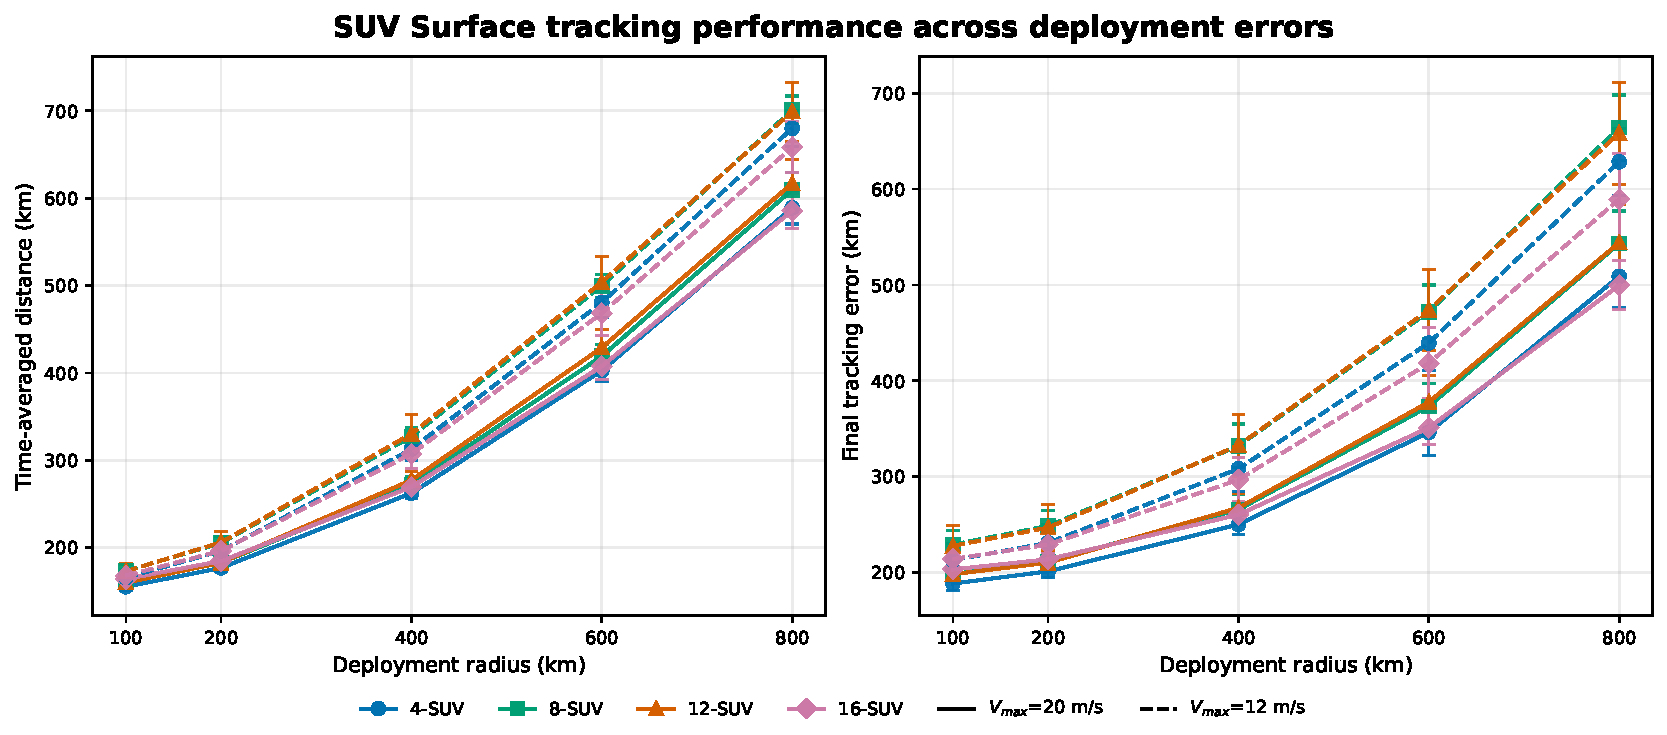
\includegraphics[width=\textwidth]
  {figures/surface_vmax_distance_comparison.pdf}
\caption{Surface tracking performance across deployment errors. The left panel
shows the fleet-mean time-averaged distance to the TC center, representing whether
the fleet remains close to the moving TC throughout an episode. The right
panel shows the final distance, representing whether the fleet reaches the TC
core by the end of the response window. Colors denote fleet sizes and line
styles denote the 20 and 12 m/s speed limits. Each point summarizes ten
independent training runs (ten random seeds), with error bars showing the
sample standard deviation.}
\label{fig:surface_vmax_comparison}
\end{figure*}
}{%
\begin{figure*}[t]
\centering
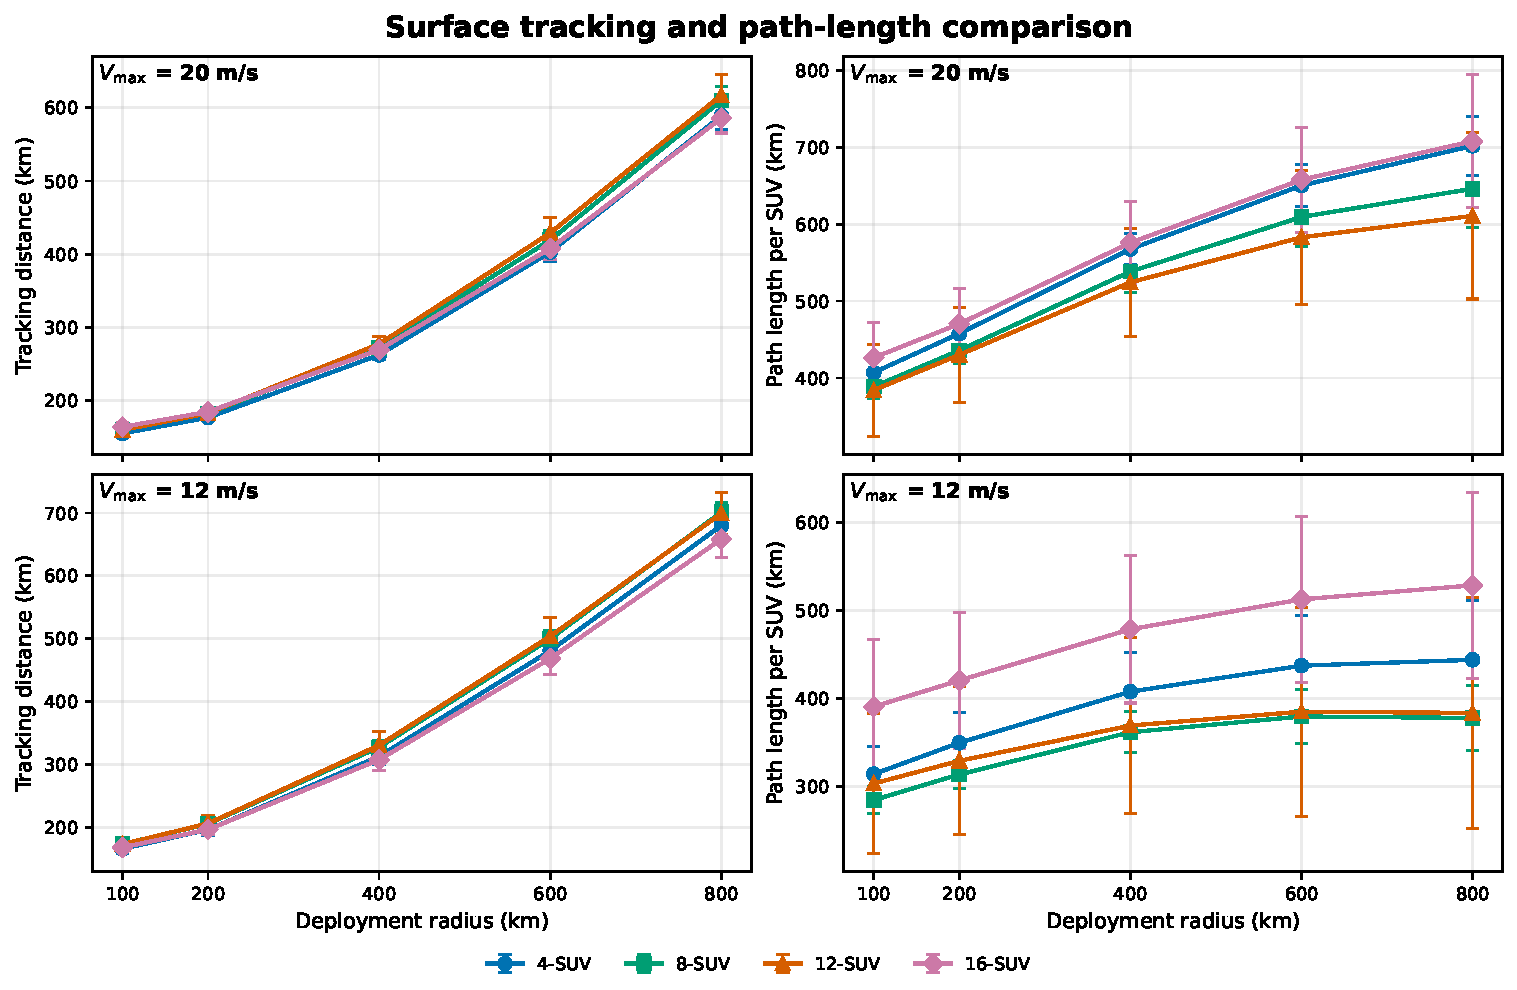
\includegraphics[width=\textwidth]
  {figures/surface_vmax_10seed_metrics.pdf}
\caption{Interim surface tracking comparison. The final version will use the
time-averaged and final TC-center distances shown in the planned two-panel
layout.}
\label{fig:surface_vmax_comparison}
\end{figure*}
}

Across the twenty matched fleet-size/radius comparisons, the 20 m/s policy has
the smaller mean time-averaged distance in all 20 cases. The median paired
difference $(d_{12}-d_{20})$ is +51.8 km. Uncorrected two-sided paired tests
indicate lower distance at 20 m/s in 19 cases and at 12 m/s in none of the
cases at $p<0.05$. Because these comparisons were not adjusted for
multiplicity, they provide exploratory rather than confirmatory evidence.

Averaged over the four fleet sizes, the differences (12 m/s minus 20 m/s) at
the five radii are: 100~km: $\Delta d=+10.1$~km, $\Delta L=-78.7$~km,
$\Delta \bar v=-1.74$~m/s; 200~km: $\Delta d=+19.3$~km,
$\Delta L=-95.5$~km, $\Delta \bar v=-2.07$~m/s; 400~km:
$\Delta d=+49.1$~km, $\Delta L=-147.4$~km, $\Delta \bar v=-3.02$~m/s;
600~km: $\Delta d=+73.5$~km, $\Delta L=-196.6$~km,
$\Delta \bar v=-3.79$~m/s; 800~km: $\Delta d=+84.2$~km,
$\Delta L=-233.3$~km, $\Delta \bar v=-4.18$~m/s. Here, positive distance and
negative path-length differences mean that the 12 m/s policy is farther from
the center and travels less; negative mean-speed differences reflect its lower
propulsion use.

The relative time-averaged distance penalty of the 12 m/s policy is 100~km:
+6.3\%; 200~km: +10.6\%; 400~km: +18.2\%; 600~km: +17.7\%; 800~km: +14.0\%.
The absolute difference therefore increases with deployment radius, although
not monotonically in relative terms. This pattern is consistent with the finite
time available to remove forecast-induced displacement. The shorter 12 m/s
paths reduce propulsion demand, but the reduced speed is associated with
weaker TC-center tracking in the tested episodes.


To provide an internally consistent visual comparison,
Figs.~\ref{fig:surface_trajectory_evolution}--\ref{fig:underwater_strategy_trajectories}
use the same held-out CHAMPI (2015) segment. The surface figures show motion
from the segment start to its endpoint, while the subsurface rollout starts
from the segment-end anchor, representing the sequential transition from
surface delivery to underwater observation.

\begin{figure*}[t]
\centering
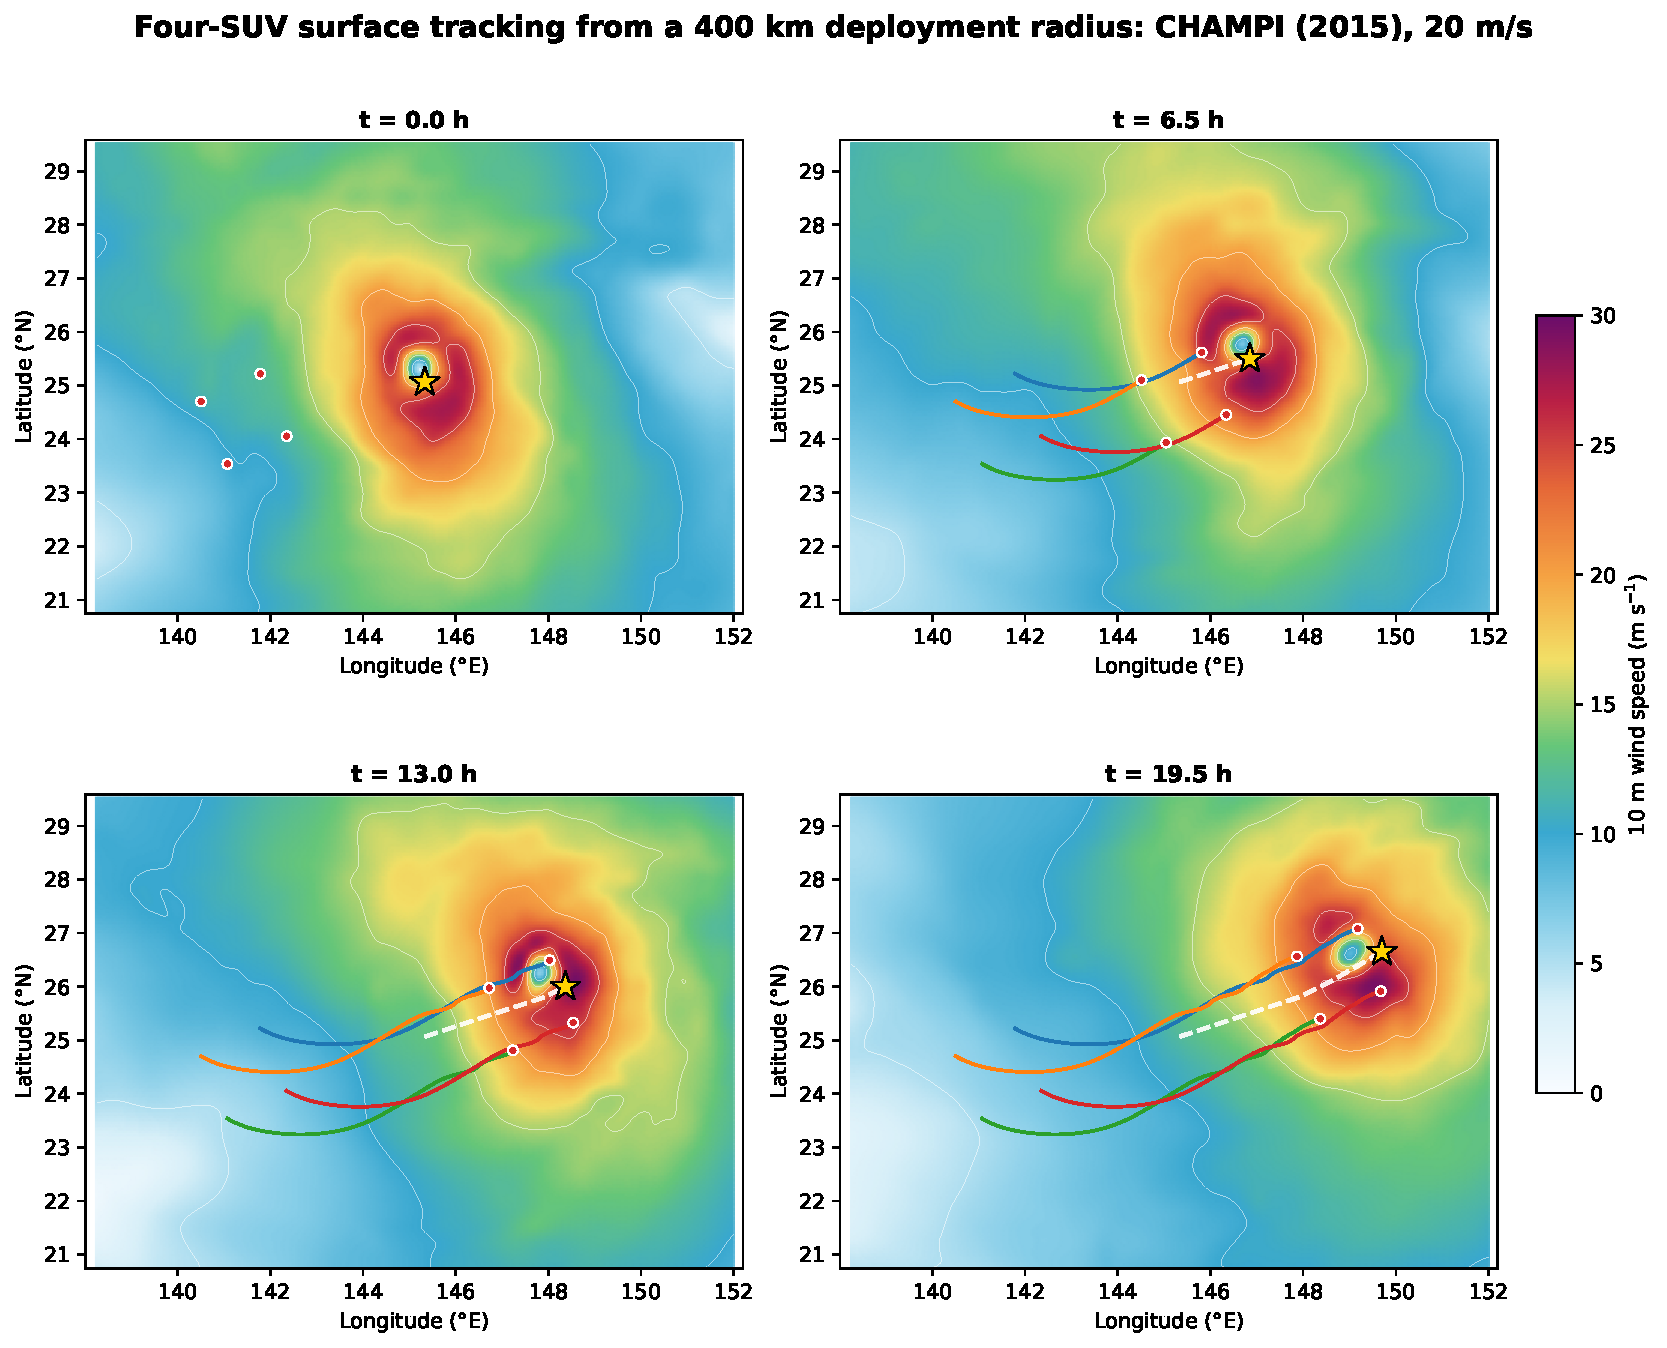
\includegraphics[width=\textwidth]
  {figures/surface_trajectory_4suv_400km_20ms.pdf}
\caption{Four-SUV surface-tracking process for CHAMPI (2015) at the 20 m/s
speed limit. The four panels show the initial deployment and subsequent
states at approximately 6.5, 13.0, and 19.5 h. The color background is the
spatially interpolated ERA5 10 m wind-speed field at each time. Small red dots
mark vehicle positions, and the yellow star marks the TC center.}
\label{fig:surface_trajectory_evolution}
\end{figure*}

Figure~\ref{fig:surface_trajectory_evolution} resolves the temporal evolution
for the four-SUV, 400 km case. At deployment, the four vehicles are dispersed
around the formation center far from the TC. During the first several hours,
the vehicles turn toward the strengthening wind region and begin to reduce the
initial displacement. By 6.5 h, all four vehicles have initiated the inward
turn; by 13.0 h they have entered the outer high-wind region; and by 19.5 h all
four trajectories have turned into the
high-wind branch and substantially reduced their initial displacement. The
individual paths differ because each vehicle has its own state and position
within the shared fleet-level wind observation; nevertheless, the fleet-level
motion follows the wind pattern toward the TC core and illustrates long-range
error correction in this representative episode.

\begin{figure*}[p]
\centering
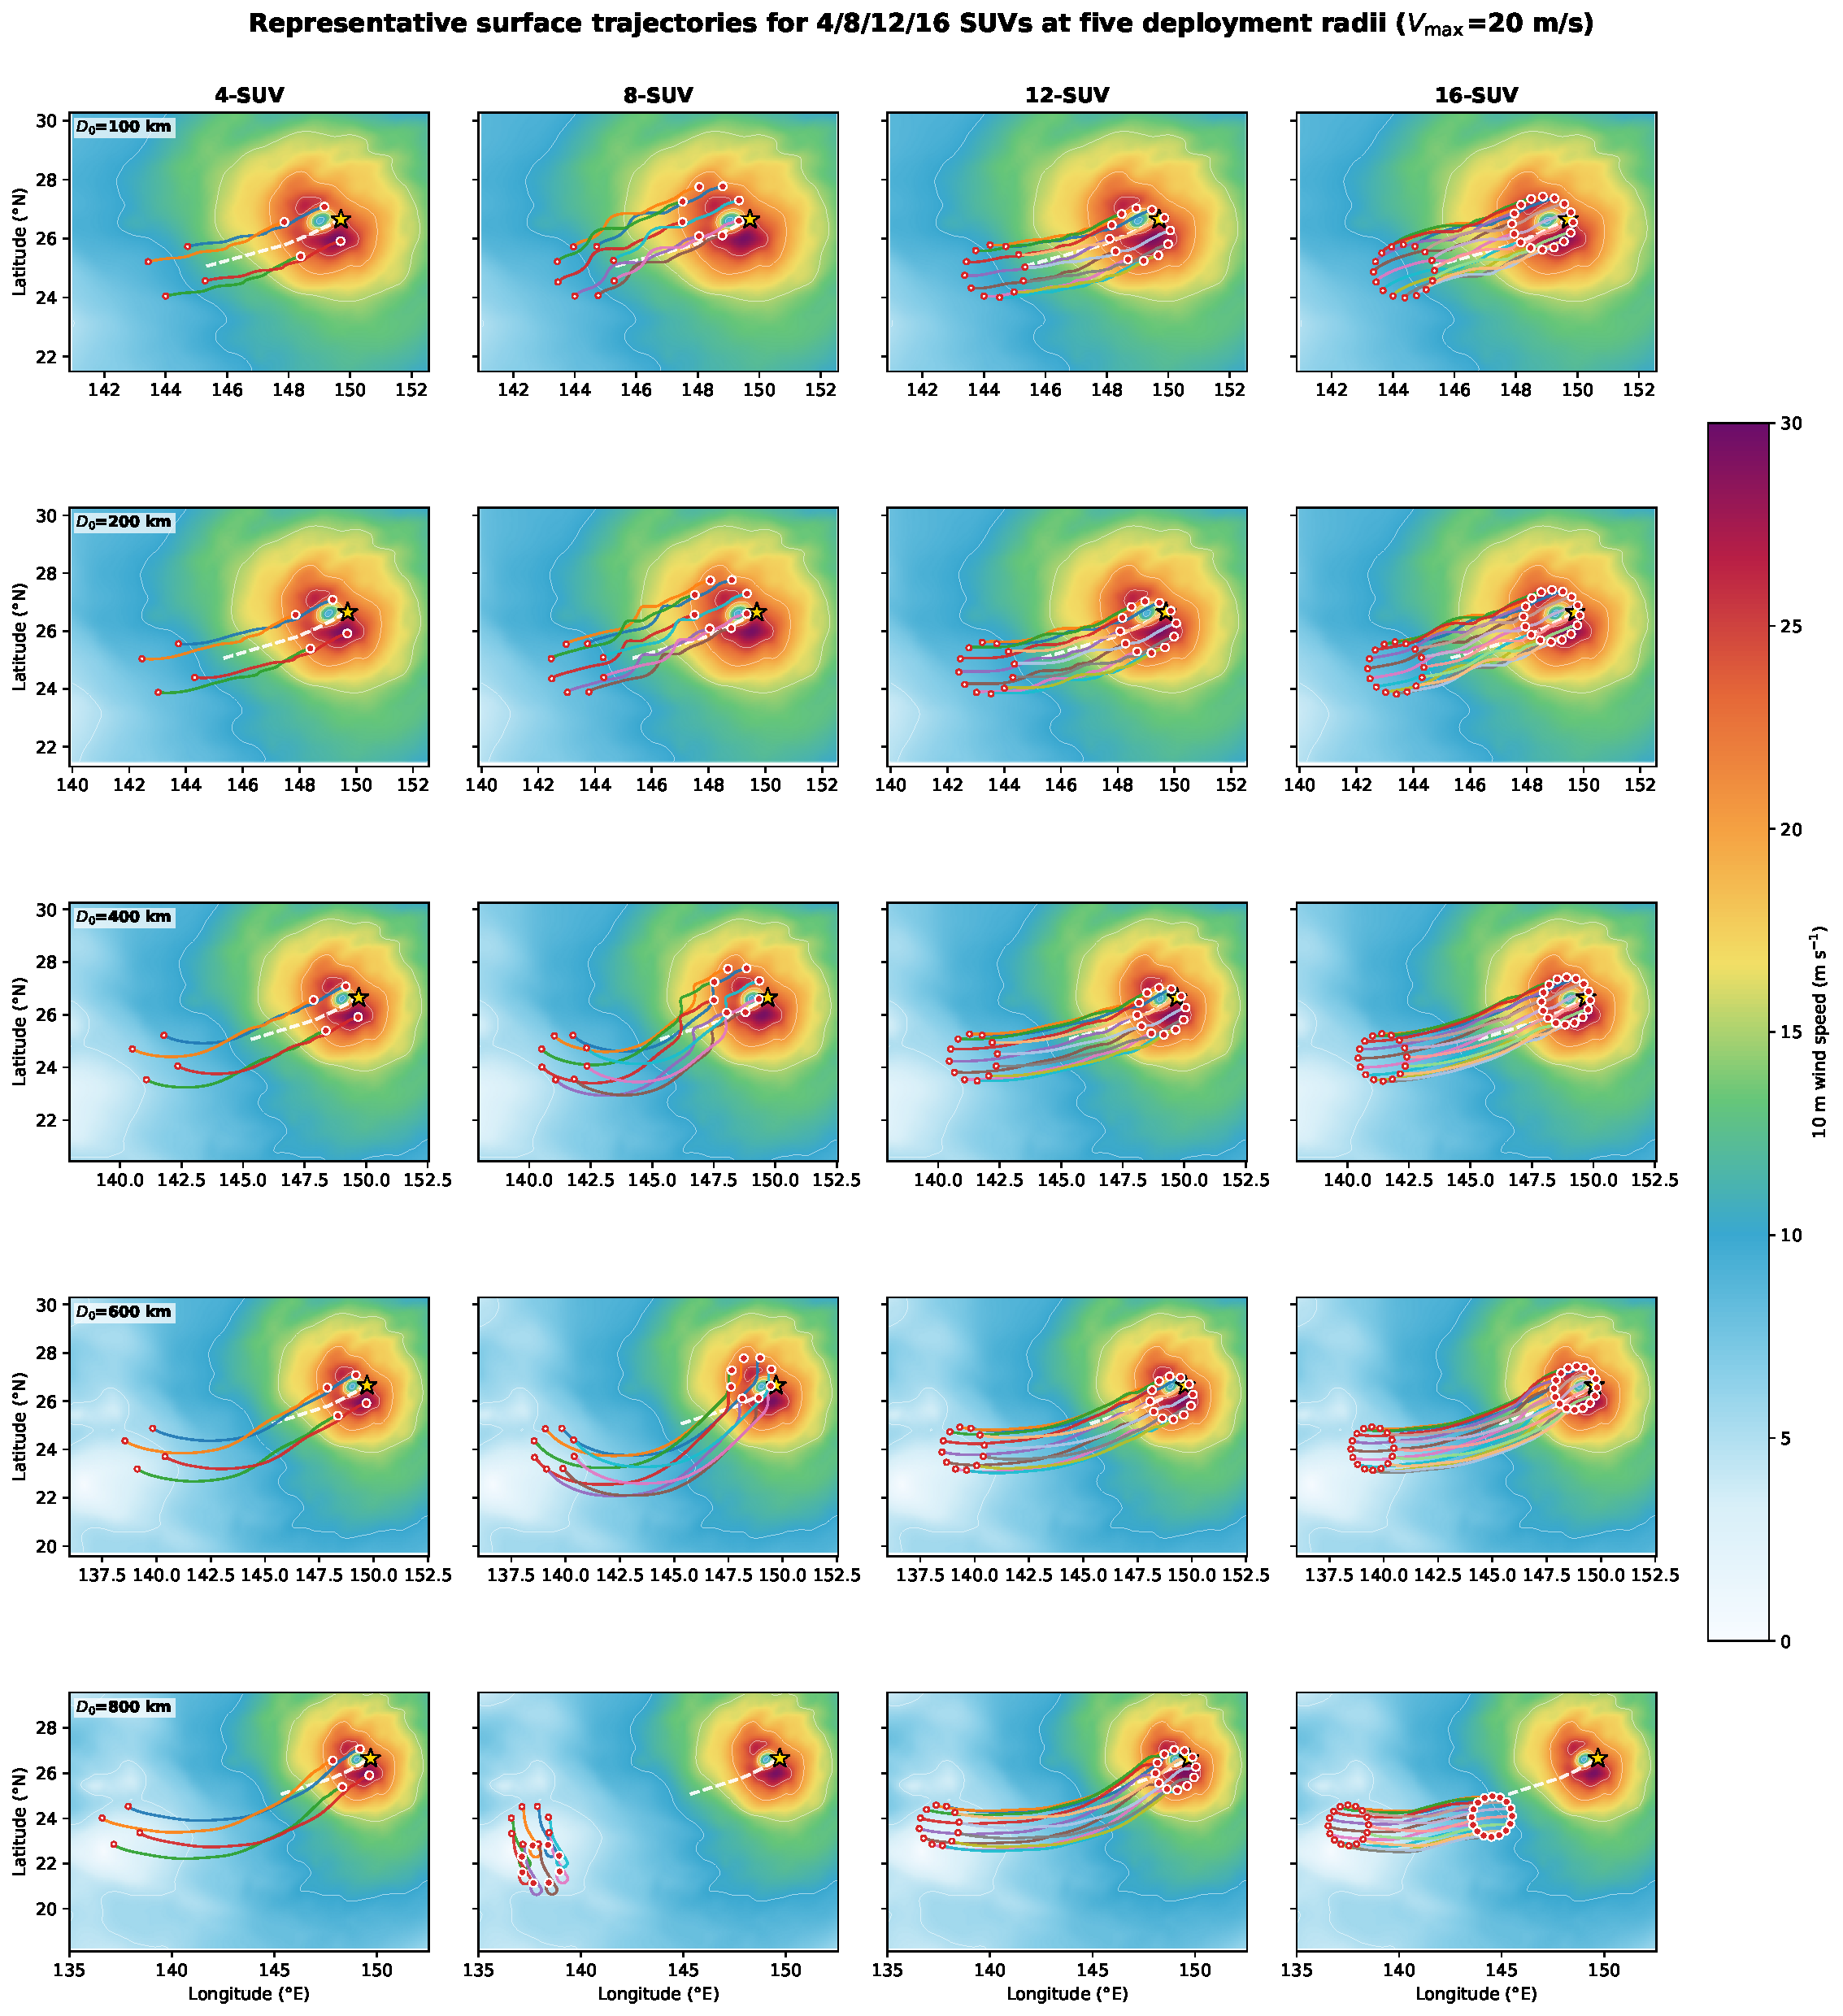
\includegraphics[width=\textwidth]
  {figures/surface_trajectory_matrix_20ms.pdf}
\caption{Representative CHAMPI (2015) trajectories for the final 20 m/s
surface policy. Columns show 4-, 8-, 12-, and 16-SUV formations, while rows
show nominal formation-center deployment radii of 100, 200, 400, 600, and
800 km. The color background is the spatially interpolated final-time ERA5
10 m wind-speed field. Thin colored lines are vehicle trajectories, open
circles mark initial positions, small red dots mark final vehicle positions,
and the yellow star marks the TC center at the end of the episode.}
\label{fig:surface_trajectory_matrix}
\end{figure*}

Figure~\ref{fig:surface_trajectory_matrix} shows how initial forecast error
changes the surface search process. At 100--200 km, the formations converge
rapidly and remain concentrated around the TC core. As the deployment radius
increases to 600--800 km, the trajectories lengthen and fan out over a wider
region before turning toward the TC. Increasing the fleet from 4 to 16 SUVs
produces a denser set of sampled branches and broader spatial coverage, but it
does not remove the need for long-range transit. In the 12- and 16-SUV cases,
many paths overlap near the core because the shared wind observations guide
the vehicles toward the same high-wind region. In these representative cases,
fleet size mainly broadens the sampled approach region, whereas deployment
error primarily determines the required transit distance.

The 600 and 800 km rows also reveal two coupled failure mechanisms at large
initial displacement. At 600 km, the representative fleet can still recover a
usable inward direction from the observed wind-speed field and its spatial
gradient, so the vehicles continue toward the TC despite the longer transit.
At 800 km, the vehicles must first overcome a larger geometric separation with
finite speed and a finite episode duration; in addition, the TC-induced wind
speed and its local gradient become weaker and less distinctive at that range.
The reduced signal quality makes the approximate bearing toward the TC more
ambiguous, so the policy may approach more slowly, change direction repeatedly,
or fail to recover the TC within the episode. These two effects are coupled:
longer travel time increases the consequence of even a small directional error,
while the weaker remote wind signature makes such an error more likely.

\subsection{Execution-Layer Action Filtering}

Table~\ref{tab:surface_control_ablations} reports the low-pass filtering
ablation over the same trained actor, 768 held-out segments, and 10 min
decision interval. Without filtering, the 4-, 8-, 12-, and 16-SUV
configurations travel 1294.9--1331.5 km per vehicle, with mean speeds of
19.23--19.73 m/s and maximum speeds of 19.92--20.00 m/s. With the
execution-layer filter ($\beta=0.8$), path length falls to 690.8--769.8 km,
mean speed to 11.11--12.72 m/s, and maximum speed to 16.13--18.20 m/s.
The fleet-mean final SUV-to-TC-center distance changes from 288.2 to 258.2 km for four SUVs,
from 305.2 to 308.6 km for eight SUVs, from 478.5 to 330.0 km for 12 SUVs, and
from 313.6 to 273.4 km for 16 SUVs. Averaged over the four fleet sizes, the
final distance decreases from 346.4 to 292.6 km, a reduction of 53.8 km
(15.5\%). Thus, filtering not only avoids degrading final tracking but improves
it on average: three fleet sizes improve, whereas the eight-SUV case increases
only slightly, by 3.4 km.

The same comparison shows reductions for every fleet size: path length
decreases by 563.4, 547.1, 618.5, and 573.6 km for 4, 8, 12, and 16 SUVs,
respectively, while maximum speed decreases by 1.80, 2.29, 3.87, and 2.94 m/s.
The 12-SUV configuration has the largest relative path-length reduction,
although the effect is not monotonic in fleet size. These results show that the
execution filter improves final tracking on average while substantially
shortening trajectories and reducing mean and peak speed.

\IfFileExists{tables/surface_control_ablations.tex}{%
\begin{table*}[htbp]
\centering
\caption{Effect of execution-layer low-pass filtering for 4/8/12/16 SUVs on the 500-TC benchmark. The same trained policy is evaluated with the filter off and on ($\beta=0.8$) on the validation dataset.}
\label{tab:surface_control_ablations}
\scriptsize
\setlength{\tabcolsep}{2.5pt}
\renewcommand{\arraystretch}{0.9}
\resizebox{0.94\textwidth}{!}{%
\begin{tabular}{@{}llrrrr@{}}
\toprule
Fleet & Filter & Final tracking error (km) & Path per SUV (km) & Mean speed (m/s) & Maximum speed (m/s) \\
\midrule
4 & Off & 288.2 & 1331.5 & 19.73 & 20.00 \\
4 & On & \textbf{258.2} & \textbf{768.1} & \textbf{12.72} & \textbf{18.20} \\
8 & Off & \textbf{305.2} & 1318.0 & 19.57 & 19.97 \\
8 & On & 308.6 & \textbf{770.9} & \textbf{12.58} & \textbf{17.68} \\
12 & Off & 478.5 & 1309.3 & 19.34 & 20.00 \\
12 & On & \textbf{330.0} & \textbf{690.8} & \textbf{11.11} & \textbf{16.13} \\
16 & Off & 313.6 & 1295.0 & 19.23 & 19.92 \\
16 & On & \textbf{273.4} & \textbf{721.4} & \textbf{11.94} & \textbf{16.98} \\
\bottomrule
\end{tabular}}
\par\smallskip
\parbox{0.94\textwidth}{\footnotesize Final tracking error is the fleet average of the individual SUV-to-best-track-center distances at the final time step. Off/on changes only the execution-layer filter on the same trained actor.}
\end{table*}

}{}

\subsection{Speed-Limit and Deployment-Error Analysis}

The 12 and 20 m/s cases answer different engineering questions. The 12 m/s
value is close to the published surface-speed scale of the current Blue Whale,
whereas 20 m/s represents a future high-speed scenario. A simple direct-pursuit
estimate illustrates why deployment radius changes the effect of this choice.
If the TC translates at speed \(U_{\mathrm{c}}\) and the SUV moves toward it at
\(V_{\max}\), the nominal closure rate is approximately
\begin{equation}
V_{\mathrm{close}}=V_{\max}-U_{\mathrm{c}}.
\label{eq:closure_speed}
\end{equation}
For a deployment error \(D\), the corresponding correction time is
\begin{equation}
t_{\mathrm{corr}}\approx\frac{D}{V_{\mathrm{close}}}.
\label{eq:correction_time}
\end{equation}
This is only a kinematic lower bound because it neglects turning and imperfect
center estimation, but it exposes the dominant scale. At 100--200 km, both
speed limits provide enough closure to correct a moderate forecast
displacement. At 600--800 km, a TC translation speed of 4--7 m/s removes a
substantial fraction of the 12 m/s speed budget. The required correction time
can then approach or exceed the 20 h mean segment duration. A 20 m/s vehicle
retains a larger reserve for reducing initial center error, but its benefit is
expected mainly at the larger radii; at short radii both cases already have
sufficient speed.

The radius-dependent pattern reported in Section~\ref{subsec:surface_results} is consistent with this
closure-rate argument. At the 800 km setting,
the mean time-averaged distances of the 20 m/s fleets are 585.6--617.0 km,
compared with 658.2--701.0 km for the 12 m/s fleets. The 12 m/s policy instead
follows a shorter path, saving 78.7--233.3 km per vehicle on average across the
five radii and operating at a lower mean speed. This is a genuine
efficiency--error trade-off: the 12 m/s scenario spends less propulsion effort
but has less ability to recover a large forecast displacement error. The gap
is relatively modest at 100--200 km, where both speed caps are adequate, and
becomes operationally material at 400--800 km.

This mechanism determines how the deployment-error curves should be read.
Differences between 12 and 20 m/s that grow with radius indicate insufficient
relative speed for forecast-error correction, whereas a similar residual error
at both speeds indicates that the limiting factor is observation information,
formation geometry, or unresolved TC motion rather than the velocity cap. The
800 km protocol is therefore conservative for the 12 m/s platform: it includes
errors that cannot always be fully removed within one segment. Operationally,
that case argues for either a faster platform, a tighter track-forecast error
envelope, or earlier deployment rather than relying on post-deployment speed
alone.

\subsection{Underwater Strategy Comparison}

The final subsurface matrix uses four SUVs and 20 h episodes. It compares
active IPPO, random control, and passive drift at ocean depths of 0, 10, 20,
30, 40, 50, and 60 m below the sea surface under maximum propulsion speeds of
1.5 and 2.0 m/s. Because the surface stage is responsible for reaching the TC
core, the underwater stage assumes that this long-range correction has already
been completed. Vehicle positions are initialized uniformly within 200 km of
the TC center, and the 100/200/400/600/800 km test-radius protocol is not
applied to the underwater policy. Passive drift exploits the TC-induced flow directly and
expends no propulsion effort. Active IPPO and random control provide the two
controlled alternatives against which the value of active propulsion is
evaluated.

Unlike the surface stage, the underwater stage assumes no inter-vehicle
communication. Each SUV conditions its action only on its own current speed,
current components, five-frame current history, and propulsion velocity. It
does not receive the observations, positions, or actions of the other SUVs.
The actor parameters are shared to ensure consistent learning across vehicles,
but information is not exchanged during execution.

Under this communication-free and decentralized formulation, increasing the
number of vehicles at a given depth would expand the aggregate sampling
footprint but would not provide any individual policy with additional
observations or decision information. The experiment was therefore designed
to test the decision strategies rather than to estimate fleet scaling
underwater. Fixing the fleet at four vehicles per depth also keeps the
active-control, random, and passive-drift comparisons paired on the same
episodes. In an actual
16-SUV deployment, the fleet can instead be divided into four groups of four,
with each group assigned to a different ocean depth. Successive groups or
deployments can then cover the seven depth layers without requiring more than
four independently acting vehicles at any one layer.

The three strategies differ only in how the propulsion command is generated:
\begin{equation}
\begin{aligned}
\mathbf a_i^{\mathrm{active}}
&=
\operatorname{clip}
\left(\pi_\theta(\mathbf o_i),-1,1\right),\\
\mathbf a_i^{\mathrm{random}}
&\sim
\mathcal U\left([-1,1]^2\right),\\
\mathbf a_i^{\mathrm{drift}}
&=
\mathbf 0.
\end{aligned}
\label{eq:underwater_policy_actions}
\end{equation}
During evaluation, the active IPPO policy uses the deterministic mean action,
whereas random control samples a new independent two-dimensional action at
every 10 min decision step. Active IPPO and random control use the same
propulsion limit and equation of motion. The active policy conditions its
action on the local current history, whereas random control ignores the
observations. Passive drift applies zero propulsion and advances solely by
ambient-current advection, so its trajectory also serves as the no-propulsion
energy baseline.

For a vehicle \(i\) assigned to depth \(z\), the ground path length after
\(K\) decision steps is
\begin{equation}
L_i(z)=\sum_{k=0}^{K-1}
\left\|\mathbf{x}_{i,k+1}-\mathbf{x}_{i,k}\right\|_2,
\label{eq:underwater_path}
\end{equation}
and the mean experienced current speed along that trajectory is
\begin{equation}
\bar V_i(z)=\frac{1}{K+1}\sum_{k=0}^{K}
\left\|\mathbf{u}_{\mathrm{ocean}}
(\mathbf{x}_{i,k},z,t_k)\right\|_2.
\label{eq:experienced_current}
\end{equation}
The figure reports the fleet-mean path length
\(N^{-1}\sum_{i=1}^{N}L_i(z)\) and the fleet-mean experienced current speed
\(N^{-1}\sum_{i=1}^{N}\bar V_i(z)\).

\begin{figure*}[t]
\centering
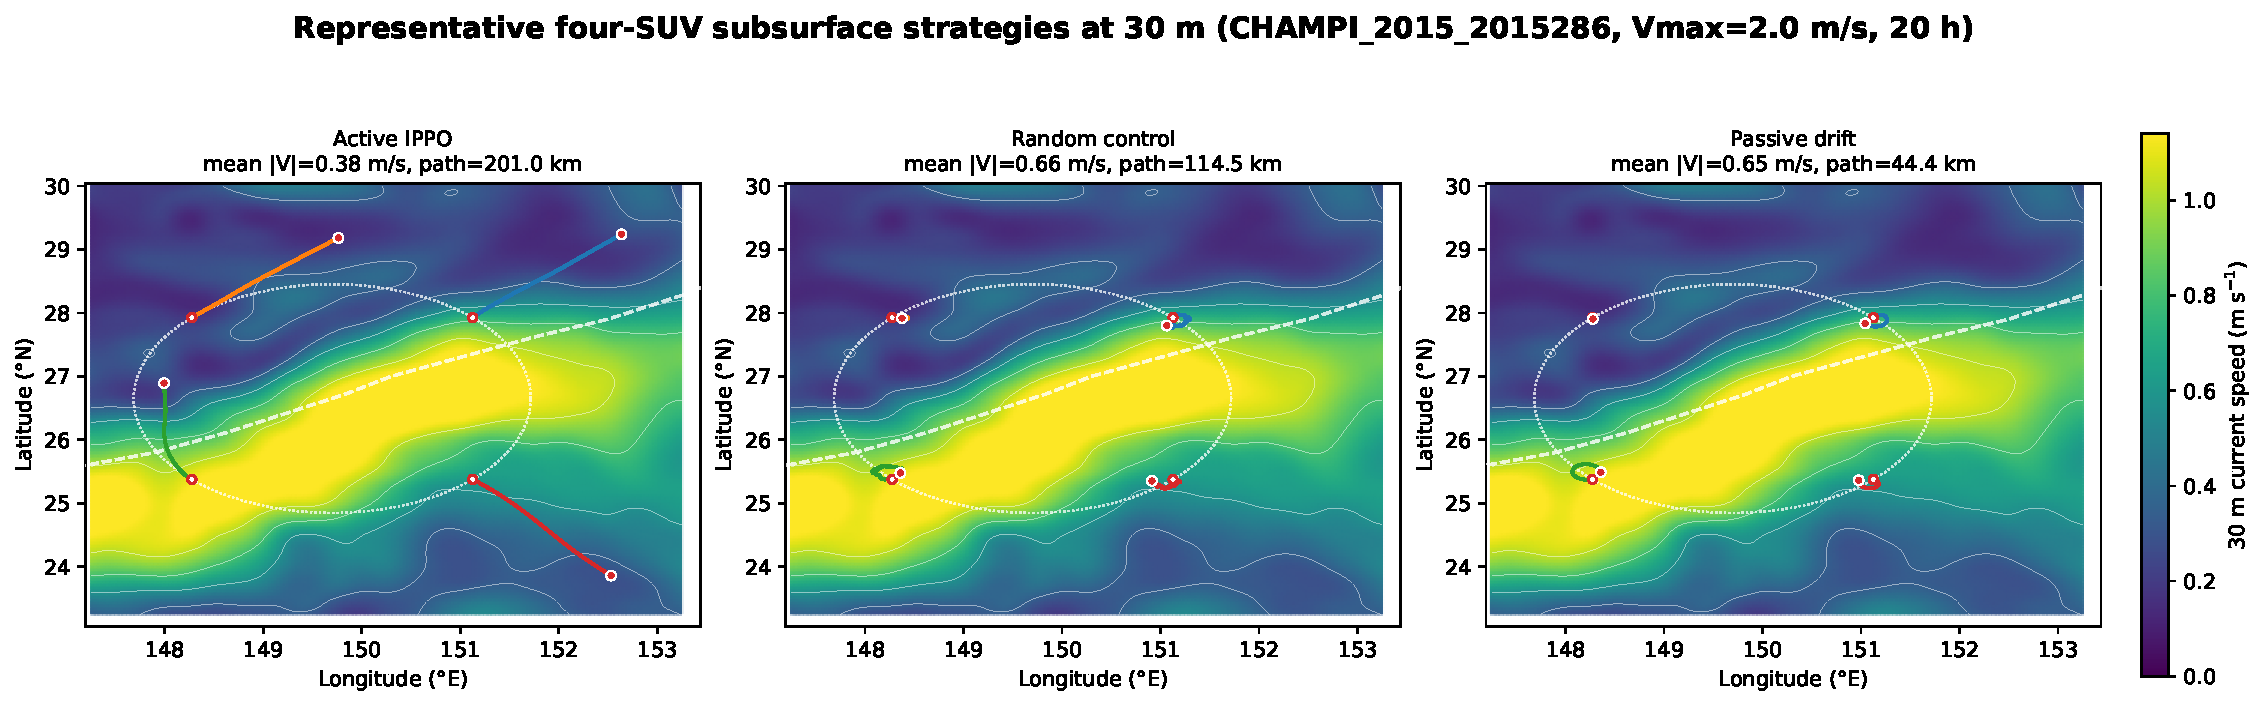
\includegraphics[width=\textwidth]
  {figures/underwater_strategy_trajectories_30m.pdf}
\caption{Representative four-SUV trajectories at 30 m depth for the same
CHAMPI (2015) segment used in the surface trajectory figures. Rollouts start
from the segment-end anchor,
under Active IPPO, random control, and passive drift. The propulsion limit is
2.0 m/s and the episode duration is 20 h. Background color is the spatially
interpolated episode-mean HYCOM current speed, dashed white curves show the TC
best track, open circles mark the four vehicles deployed with 90$^\circ$
spacing on a 200 km initial ring, and small red dots mark final vehicle
positions. This episode is illustrative and is not used for the final
comparative statistics.}
\label{fig:underwater_strategy_trajectories}
\end{figure*}

Figure~\ref{fig:underwater_strategy_trajectories} illustrates the qualitative
trajectory construction for the three strategies. It is retained as a
qualitative example only; all comparative inference is deferred to the final
ten-seed, seven-depth evaluation.

\IfFileExists{figures/underwater_methods_7depth.pdf}{%
\begin{figure*}[t]
\centering
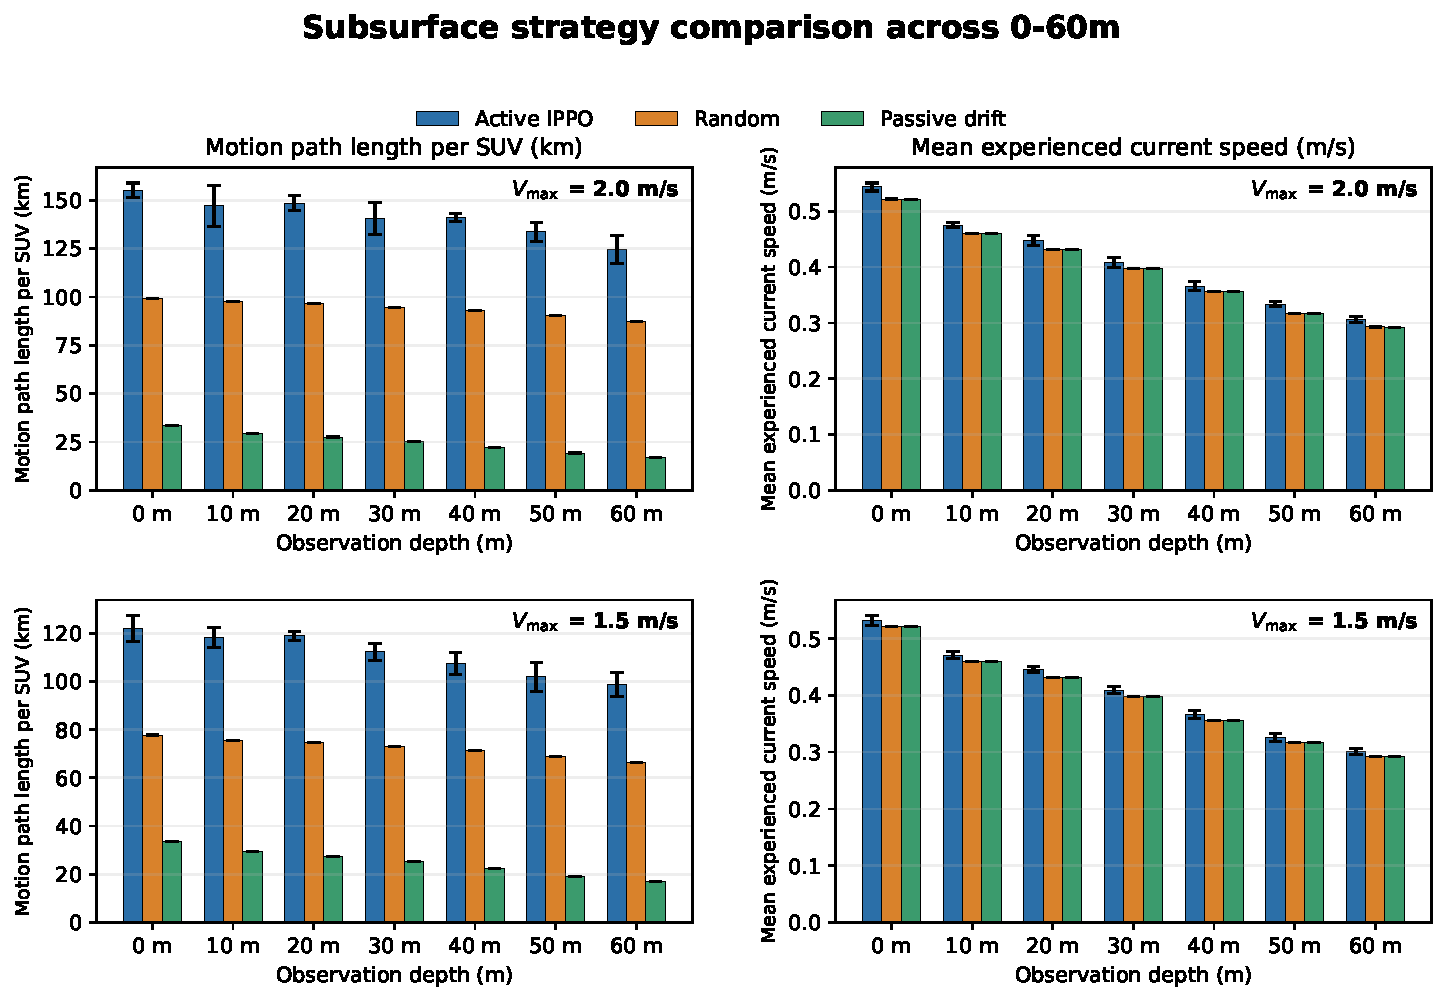
\includegraphics[width=\textwidth]
  {figures/underwater_methods_7depth.pdf}
\caption{Ten-seed comparison of active control, random control, and passive
drift in the 20 h subsurface task at seven depths from 0 to 60 m. Rows show
maximum propulsion speeds of 2.0 and 1.5 m/s; columns report the fleet-mean
motion path length and mean experienced current speed. Error bars show the
sample standard deviation across ten active-policy training seeds. Random
control and passive drift are paired baselines without training-seed
variability.}
\label{fig:underwater_methods_10seed}
\end{figure*}
}{%
\IfFileExists{figures/underwater_methods_7depth_preview.pdf}{%
\begin{figure*}[t]
\centering
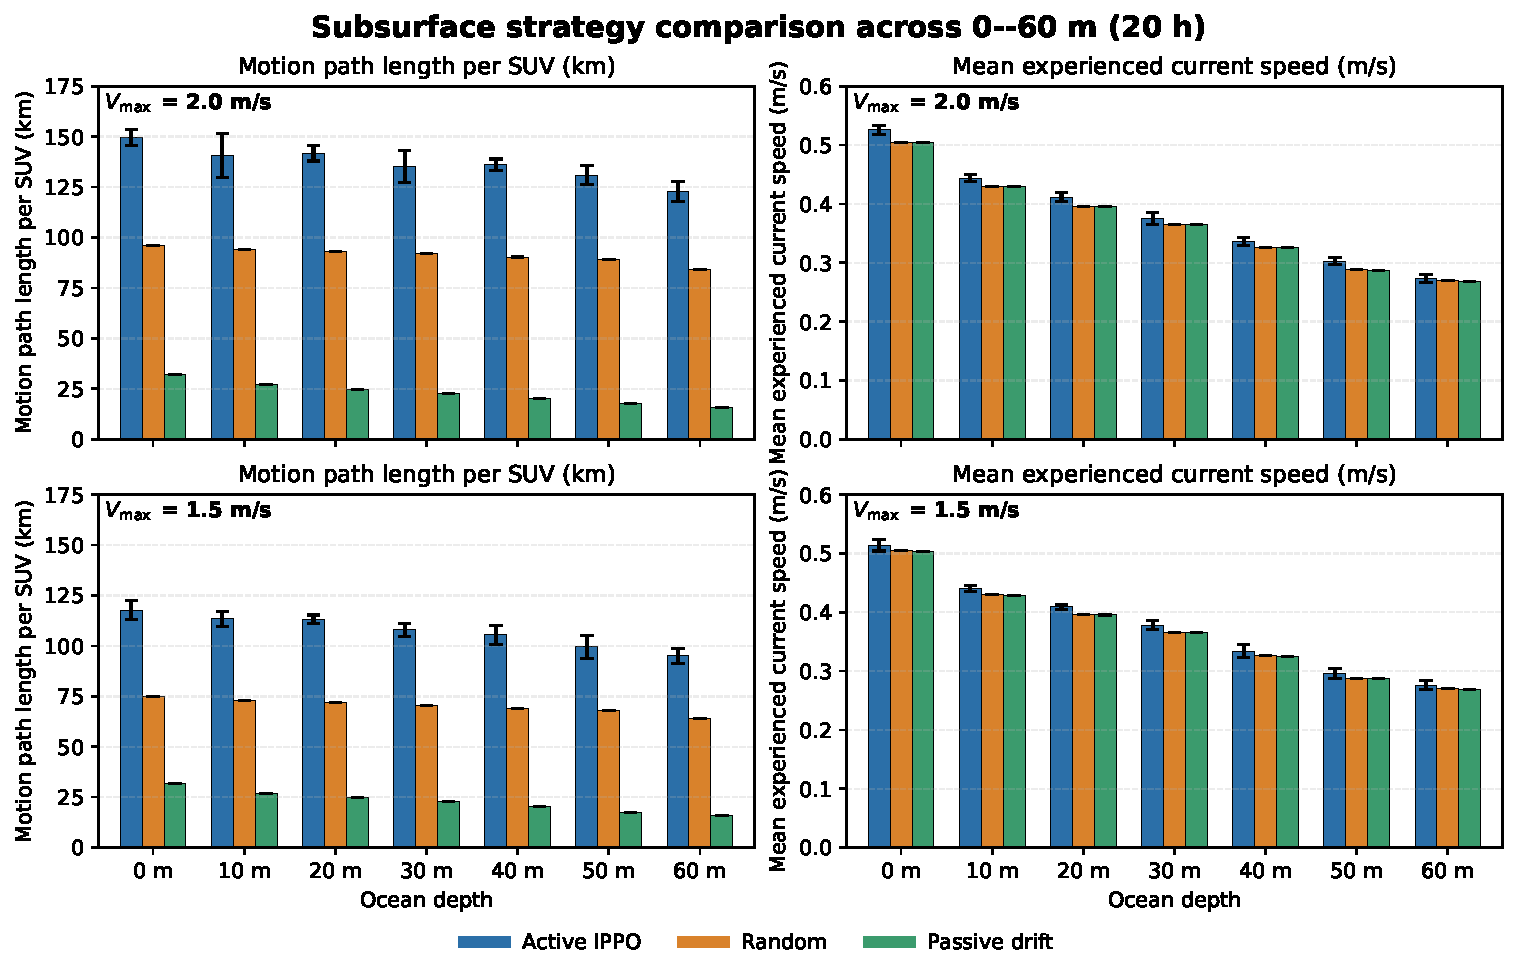
\includegraphics[width=\textwidth]
  {figures/underwater_methods_7depth_preview.pdf}
\caption{Preview of the planned seven-depth comparison at maximum propulsion
speeds of 2.0 and 1.5 m/s. Columns show the fleet-mean motion path length and
mean experienced current speed. Axes and legends define the final layout; no
experimental values are plotted until all ten-seed seven-depth results are
available.}
\label{fig:underwater_methods_10seed}
\end{figure*}
}{%
\IfFileExists{figures/underwater_methods_10seed.pdf}{%
\begin{figure*}[t]
\centering
\includegraphics[width=\textwidth]
  {figures/underwater_methods_10seed.pdf}
\caption{Interim ten-seed comparison at the currently available 0, 30, and
50 m depths.}
\label{fig:underwater_methods_10seed}
\end{figure*}
}{}%
}%
}{}

Figure~\ref{fig:underwater_methods_10seed} defines the layout of the final
seven-depth comparison and will be populated only after all ten-seed active
policies have been retrained and evaluated under the corrected implementation.
No quantitative underwater ranking is inferred from the present placeholder.

This behavior is consistent with the speed scales in the near-core region. For the
paired 20 h episodes initialized within 200 km of the TC center, the
area-averaged current speed at the evaluated 0, 30, and 50 m depths is
0.34--0.57 m/s, while the spatial 95th percentiles are 0.92--1.30 m/s and the
99th percentiles are 1.30--1.85 m/s. Strong local-current maxima reach
2.19--3.55 m/s across these depths, and the average local maximum within an
instantaneous 200 km core area is 0.91--1.24 m/s. Thus, the high-current tail
and local maxima are comparable to, or even exceed, the SUV propulsion limits
of 1.5 and 2.0 m/s. This similarity in scales motivates the active-versus-drift
comparison but does not by itself establish which strategy is preferable.
Active propulsion can relocate a vehicle, whereas passive drift follows the
ambient flow at zero propulsion effort; the final matrix will quantify the
resulting differences in experienced current speed, coverage, ground path,
and mean ground speed.

\IfFileExists{figures/underwater_energy_path_vs_depth.pdf}{%
\begin{figure*}[t]
\centering
\includegraphics[width=\textwidth]
  {figures/underwater_energy_path_vs_depth.pdf}
\caption{Comparison of propulsion energy and path length across the seven
subsurface observation depths. Each column corresponds to one maximum
propulsion speed, and each line compares active IPPO, random control, and
passive drift. The energy ordinate is the propulsion proxy \(E_3\), and shaded
regions denote the standard error across evaluation seeds.}
\label{fig:underwater_energy_path}
\end{figure*}
Figure~\ref{fig:underwater_energy_path} separates the propulsion proxy from
the corresponding ground path across depths and speed limits. It is interpreted
only as a relative computational proxy, not as measured electrical energy.
}{}

\section{Conclusion}

This paper presented a simulation-based multi-agent reinforcement learning
(MARL) framework using IPPO for coordinated surface--subsurface observation of
tropical cyclones with parameterized Blue Whale-class SUVs. Event-specific
simulation environments were constructed from 500 historical TCs, with 450 TCs
used for training and 50 for testing. ERA5 winds, HYCOM currents at seven
depths from 0 to 60 m, and IBTrACS tracks were aligned into a common
event-specific environment. Surface experiments covered 4-, 8-, 12-, and
16-SUV fleets, 12 and 20 m/s speed limits, ten seeds, and deployment errors
from 100 to 800 km. Surface vehicles shared their wind observations across the
fleet. After entering the 200 km near-core region, underwater vehicles used
propulsion limits of 1.5 and 2.0 m/s without inter-vehicle communication.

The surface results support an asymmetric surface operating strategy: 20 m/s
improved long-range error correction, whereas 12 m/s reduced path length and
mean speed but left a larger residual tracking error. Low-pass filtering
improved final tracking on average while further reducing path length and peak
speed. These results also show the intended observation--planning coupling:
surface measurements continuously alter the next motion command rather than
only populating a post hoc map. The underwater evaluation is configured to compare
active IPPO, random control, and passive drift across all seven depths under
the corrected unit-disk action and causal five-frame observation
implementation; final quantitative conclusions are deferred until this matrix
is complete. The present evidence is simulation-based and uses a mission-level
horizontal point-mass approximation; no field validation or operational
forecast impact is claimed. Future work should couple the planner to
calibrated six-degree-of-freedom vehicle dynamics and evaluate the resulting
observations in air--sea coupled data assimilation.




\section*{Code and package availability}
\begin{sloppypar}
The final experiment code, simulation environments, evaluation scripts, and
processed result tables are available at
\url{https://github.com/DYHAI/SUV-MARL-TC}. The experiments used
Python 3.11, Stable-Baselines3 2.9.0, Gymnasium 1.2.2,
PyTorch 2.11.0+cu128, NumPy 2.4.6, pandas 2.3.3,
xarray 2026.7.0, SciPy 1.17.1, and Matplotlib 3.11.1.
Training and evaluation were performed on a workstation with a 24-core
Intel Core Ultra 7 270K Plus CPU, 64 GB DDR5 memory, and an NVIDIA RTX 5060 Ti
16 GB GPU.
\end{sloppypar}

\section*{Acknowledgements}
This project is supported by the National Natural Science Foundation of China (42530402 and 42227901),  the China Postdoctoral Science Foundation (2025M783467), the Project of State Key Laboratory of Satellite Ocean Environment Dynamics (SOEDZZ2527) and Innovation Group Project of Southern Marine Science and Engineering Guangdong Laboratory (Zhuhai) (311024004).











\printcredits

\clearpage
\onecolumn
\appendix

\section{Reward and IPPO Hyperparameters}\label{app:parameters}

\setcounter{table}{0}
\renewcommand{\thetable}{A.\arabic{table}}

Table~\ref{tab:reward_parameters} summarizes the reward, action-filter, and
safety parameters used in the surface and underwater experiments.
Table~\ref{tab:ippo_hyperparams} lists the shared IPPO network and training
hyperparameters.

% ============================================================
% Table A.1: Merged reward and safety parameters
% ============================================================
\begin{center}
\small
\captionof{table}{Reward, action-filter, and safety parameters used in the final
surface and underwater experiments.}
\label{tab:reward_parameters}
\resizebox{\textwidth}{!}{%
\begin{tabular}{@{}p{0.18\textwidth}p{0.12\textwidth}p{0.15\textwidth}p{0.45\textwidth}@{}}
\toprule
Parameter & Symbol & Value & Description and applicable task \\
\midrule
\multicolumn{4}{l}{\textbf{Panel A: surface reward and controller parameters}} \\
Proximity-cost distance cap & $D_{\max}$ & 300 km &
Distance cost is capped at 300 km to prevent excessively large gradients
from distant initial deployments. \\
Near-center threshold & $d_{\mathrm{near}}$ & 100 km &
Threshold defining the discrete near-center bonus. \\
Near-center bonus & $b_{\mathrm{near}}$ & 1.0 &
Bonus assigned when an SUV is within 100 km of the TC center. \\
Radius-excess threshold & $R_{\mathrm{form}}$ & 100 km &
Reference radius used by the additional distance penalty beyond 100 km. \\
Radius-excess weight & $W_{\mathrm{form}}$ & 1.0 &
Weight of the penalty applied when an individual SUV is farther than 100 km
from the TC center. \\
Action-change weight & $\lambda_u$ & 0.05 &
Weight of the squared action change
$\|\mathbf{a}_{i,t}-\mathbf{a}_{i,t-1}\|_2^2$ at the 10 min interval. \\
Action-filter coefficient & $\beta_{\mathrm{filt}}$ & 0.8 &
Coefficient of
$\mathbf{a}_t^{\mathrm{filt}}=
(1-\beta)\mathbf{a}_t^{\mathrm{raw}}
+\beta\mathbf{a}_{t-1}^{\mathrm{filt}}$.
This is a controller setting rather than a reward term. \\
Surface reward clipping range & $[r_{\min},r_{\max}]$ & $[-5,2]$ &
Clipping range applied to the team-averaged surface reward. \\

\midrule
\multicolumn{4}{l}{\textbf{Panel B: underwater active-control comparison parameters}} \\
Current-speed normalization & $V_{\mathrm{norm}}$ & 1.0 m/s &
Current-intensity reward is implemented as
$\min(\|\mathbf{u}\|/V_{\mathrm{norm}},R_{\max})$. \\
Current-reward cap & $R_{\max}$ & 2.0 &
Upper bound of the normalized current-speed reward. \\
Propulsion-energy weight & $\lambda_E$ & 0.05 &
Weight of the propulsion penalty
$\lambda_E\|\tilde{\mathbf{a}}_i\|_2^2$ in the current-seeking reward. \\
Downstream-alignment weight & $\beta_{\parallel}$ & 0.5 &
Weight of the positive propulsion--current alignment term. \\
Underwater reward clipping range & $[r_{\min},r_{\max}]$ & $[-5,5]$ &
Clipping range applied to the team-averaged underwater reward during active
control training. \\

\midrule
\multicolumn{4}{l}{\textbf{Panel C: shared coastal-safety parameters}} \\
Land penalty & $P_{\mathrm{land}}$ & 20 &
Penalty applied when an SUV enters a land cell. Shared by the surface and
underwater environments. \\
Nearshore buffer distance & $D_{\mathrm{buf}}$ & 100 km &
Width of the soft nearshore safety buffer. \\
Nearshore penalty weight & $W_b$ & 8.0 &
Maximum soft-penalty weight within the 100 km nearshore buffer. \\
Minimum deployment offshore distance & $D_{\mathrm{deploy}}$ & 100 km &
Minimum coastline distance required by offshore-only rejection sampling during
deployment. \\
Action-filter safety margin & $D_{\mathrm{filter}}$ & 100 km &
Distance below which the onshore component of the commanded action is removed. \\
\bottomrule
\end{tabular}}
\par\smallskip
\parbox{\textwidth}{\footnotesize
Note: the final subsurface comparison consists of active IPPO, random control,
and passive drift. Passive drift does not optimize a learned propulsion policy
or reward.}
\end{center}

\clearpage

% ============================================================
% Table A.2: IPPO hyperparameters
% ============================================================
\begin{center}
\footnotesize
\captionof{table}{Parameter-sharing IPPO network and training hyperparameters
used in the final surface and subsurface comparisons.}
\label{tab:ippo_hyperparams}
\resizebox{\textwidth}{!}{%
\begin{tabular}{@{}p{0.18\textwidth}p{0.13\textwidth}p{0.17\textwidth}p{0.42\textwidth}@{}}
\toprule
Parameter & Symbol & Value & Description \\
\midrule
Algorithm & -- & PPO &
Stable-Baselines3 PPO with parameter sharing and independent per-agent action
sampling. \\
Return aggregation & -- & Team average &
The environment reward is averaged across the $N$ SUVs before computing the
shared PPO return. \\
Optimizer & -- & Adam &
Adam optimizer used for the actor and critic parameters. \\
Policy network & -- & $2\times256$ MLP &
Actor: Linear($d_{\mathrm{obs}},256$)--Tanh--
Linear($256,256$)--Tanh--Linear($256,d_{\mathrm{act}}$). \\
Value network & -- & $2\times256$ MLP &
Critic: Linear($d_{\mathrm{obs}},256$)--Tanh--
Linear($256,256$)--Tanh--Linear($256,1$).
Per-agent values are summed during training. \\
Per-agent observation dimension & $d_{\mathrm{obs}}$ & 14/26/38/50 &
Surface wind-only observations for 4/8/12/16 SUVs, respectively. The
four-SUV underwater active-control comparison uses $d_{\mathrm{obs}}=17$. \\
Surface observation & -- & Wind at 10 m above sea level &
Using ideal surface communication, each SUV receives the current wind speed and
components at 10 m above the sea surface observed by every SUV in the fleet. \\
Underwater observation & -- & Current only &
With no inter-vehicle communication, the active IPPO controller observes only
its own local current speed and components at the assigned ocean depth, together
with a five-frame history and its own normalized propulsion velocity. \\
Action dimension & $d_{\mathrm{act}}$ & 2 per SUV &
Continuous east--north velocity command in $[-1,1]^2$, followed by circular
projection to enforce the maximum-speed constraint. \\
Parallel environments & $N_{\mathrm{env}}$ & 4 &
Number of vectorized training environments. \\
Rollout length & $n_{\mathrm{steps}}$ & 2048 &
Number of steps collected per environment before each PPO update. \\
Mini-batch size & $B$ & 256 &
Mini-batch size used during each gradient update. \\
Optimization epochs & $N_{\mathrm{epochs}}$ & 10 &
Number of passes over each rollout. \\
Learning rate & $\alpha$ & $3\times10^{-4}$ &
Adam learning rate used for the actor and critic. \\
Discount factor & $\gamma$ & 0.99 &
Reward discount factor. \\
GAE parameter & $\lambda_{\mathrm{GAE}}$ & 0.95 &
Generalized advantage estimation applied to the team-average reward. \\
Policy clipping range & $\epsilon$ & 0.2 &
Clipping range of the PPO probability ratio. \\
Value clipping range & $\epsilon_v$ & 0.2 &
Clipping range of the value-function update. \\
Entropy coefficient & $c_{\mathrm{ent}}$ & 0.01 &
Entropy regularization coefficient. \\
Value-loss coefficient & $c_v$ & 0.5 &
Weight of the value-function loss. \\
Maximum gradient norm & $g_{\max}$ & 0.5 &
Global gradient clipping threshold. \\
Training steps & $T$ & $2\times10^6$ &
Nominal environment steps per training run. \\
Independent seeds & -- & 0--9 &
Ten random seeds for each selected surface or active-control configuration. \\
Surface training forecast-error radius & $R_{\mathrm{train}}$ & 0--800 km &
The surface formation-center offset is sampled uniformly inside the 800 km
disk around the initial TC center; both bearing and radial distance are
randomized. This models the assumed upper bound of TC track-forecast error. \\
Surface validation center offsets & $R_{\mathrm{test}}$ &
100/200/400/600/800 km &
Fixed surface formation-center offsets with random bearings, evaluated without
retraining. These values represent increasing track-forecast displacement. \\
Underwater initialization radius & $R_{0,\mathrm{u}}$ & $\leq$200 km &
After surface convergence, subsurface vehicles are initialized uniformly
within 200 km of the TC center. The 0--800 km forecast-error protocol is
surface-only. \\
Decision interval & $\Delta t$ & 10 min &
Environmental observation and action interval. \\
Surface formation radius & $R_{\mathrm{ring}}$ & 100 km &
Surface SUVs use equal angular spacing of \(360^\circ/N\) on a 100 km ring. \\
Surface fleet sizes & $N$ & 4/8/12/16 &
Number of SUVs in the final surface configurations. \\
Underwater fleet size & $N$ & 4 &
Number of SUVs in each active-IPPO, random-control, and passive-drift case. \\
Underwater depths below the sea surface & $z$ &
0/10/20/30/40/50/60 m &
Seven ocean-current observation depths used in the final subsurface matrix. \\
Underwater methods & -- & Active IPPO; random; drift &
Three paired methods evaluated on the same episodes and deployments. \\
Underwater duration & $H$ & 20 h &
Fixed mission window for the final subsurface comparison. \\
Surface speed limits & $V_{\max}^{\mathrm{s}}$ & 12 or 20 m/s &
Two surface-speed scenarios. \\
Submerged speed limits & $V_{\max}^{\mathrm{u}}$ & 1.5 or 2.0 m/s &
Two resultant propulsion-speed limits after unit-disk action projection,
used for the active-control comparison. \\
Compute device & -- & CPU &
All reported PPO/IPPO experiments were trained on CPU. \\
\bottomrule
\end{tabular}}
\end{center}

\clearpage
\twocolumn
\bibliographystyle{elsarticle-num}
\bibliography{MARL_Ding}



%\vskip3pt

% \bio{}
% Author biography without author photo.
% Author biography. Author biography. Author biography.
% Author biography. Author biography. Author biography.
% Author biography. Author biography. Author biography.
% Author biography. Author biography. Author biography.
% Author biography. Author biography. Author biography.
% Author biography. Author biography. Author biography.
% Author biography. Author biography. Author biography.
% Author biography. Author biography. Author biography.
% Author biography. Author biography. Author biography.
% \endbio

% \bio{figs/pic1}
% Author biography with author photo.
% Author biography. Author biography. Author biography.
% Author biography. Author biography. Author biography.
% Author biography. Author biography. Author biography.
% Author biography. Author biography. Author biography.
% Author biography. Author biography. Author biography.
% Author biography. Author biography. Author biography.
% Author biography. Author biography. Author biography.
% Author biography. Author biography. Author biography.
% Author biography. Author biography. Author biography.
% \endbio

% \bio{figs/pic1}
% Author biography with author photo.
% Author biography. Author biography. Author biography.
% Author biography. Author biography. Author biography.
% Author biography. Author biography. Author biography.
% Author biography. Author biography. Author biography.
% \endbio

\end{document}
